\chapter{Hasil Implementasi dan Pembahasan}

Bab ini menyajikan hasil implementasi, evaluasi empiris, dan analisis mendalam sistem \textit{automated web penetration testing} berbasis \textit{Reinforcement Learning} (RL) yang telah dirancang pada Bab 3. Pengujian difokuskan pada evaluasi performa dua algoritma pemelajaran penguatan, yaitu algoritma tabular \textit{Q-Learning} dan algoritma aproksimasi fungsi mendalam \textit{Deep Q-Network} (DQN), terhadap aplikasi target \textit{OWASP Juice Shop}. Selain itu, bab ini juga menyajikan evaluasi detektor terhadap \textit{ground truth} hasil kurasi manual untuk memutus sirkularitas metrik, analisis mekanisme gerbang kualitas eksploitasi nyata, dinamika transisi eksplorasi-eksploitasi, perbandingan komparatif mendalam Q-Learning terhadap DQN, serta perbandingan efisiensi \textit{apples-to-apples} dengan pemindai kerentanan konvensional \textit{OWASP ZAP}.

\section{Pengumpulan dan Pengolahan Data}

Tahap pengumpulan dan pengolahan data merupakan landasan empiris dalam mengevaluasi efektivitas sistem \textit{automated web penetration testing} berbasis \textit{Reinforcement Learning}. Bagian ini menguraikan secara komprehensif mengenai prosedur perolehan data interaksi HTTP dari lingkungan target, skema atribut data yang direkam, tahapan pembersihan dan penapisan data, transformasi fitur respons ke dalam ruang representasi model, serta formulasi agregasi metrik kuantitatif yang digunakan dalam analisis kinerja.

\subsection{Prosedur Pengumpulan Data Eksperimen}

Pengumpulan data dilakukan secara otomatis melalui interaksi terprogram antara sistem pengetesan penetrasi dengan aplikasi target \textit{OWASP Juice Shop} v20.2.0 pada lingkungan lokal terisolasi (\texttt{http://localhost:3000}). Data yang dikumpulkan bersumber dari empat instrumen pengujian:
\begin{enumerate}
    \item \textbf{Data Penyelidikan Baseline (\textit{Baseline Probing Data}):} Sebelum fase pelatihan dimulai, sistem mengirimkan satu permintaan HTTP berstatus netral (\texttt{"hello"}) ke setiap \textit{endpoint} (total 8 transaksi). Data respons (khususnya ukuran panjang badan respons dalam satuan byte) direkam untuk membentuk nilai acuan awal (\textit{endpoint baseline length}).
    \item \textbf{Data Transaksi Pelatihan Reinforcement Learning:} Pengumpulan data primer dilakukan selama $1.585$ episode pengujian per agen (total $3.170$ transaksi muatan uji untuk Q-Learning dan DQN). Pada setiap episode, agen mentransmisikan satu muatan uji terpilih melalui modul \texttt{HTTPClient}, lalu mencatat seluruh metadata respons server yang diterima.
    \item \textbf{Data Verifikasi Kualitas Eksploitasi:} Setiap kali terdeteksi indikasi kerentanan aktif, sistem secara otomatis merekam data transaksi tambahan:
    \begin{itemize}
        \item Untuk SQL Injection dan Fuzzing, modul pengujian mengirimkan probe kontrol netral dan mutan ternetralkan (tercatat 47 transaksi verifikasi pada Q-Learning dan 43 transaksi pada DQN). 
        \item Untuk XSS, modul \texttt{BrowserVerifier} memuat peramban \textit{Playwright Chromium} tanpa antarmuka untuk mengeksekusi muatan pada DOM (tercatat 30 kali navigasi peramban pada Q-Learning dan 28 kali pada DQN). 
    \end{itemize}
    \item \textbf{Data Pemindaian Pembanding OWASP ZAP:} Data pembanding diperoleh dari eksekusi pemindaian terkontrol (\textit{controlled scan}) menggunakan OWASP ZAP v2.15 pada dua \textit{endpoint} bersama (\texttt{/rest/products/search?q=} dan \texttt{/ftp/}). Seluruh riwayat pesan HTTP (1.585 pesan) dan daftar peringatan keamanan (\textit{alerts}) diekstraksi melalui antarmuka \textit{ZAP Core API}.
\end{enumerate}

Seluruh data transaksi interaksi agen dicatat secara serial dan persisten ke dalam berkas log terstruktur berformat \textit{Comma-Separated Values} (\texttt{log\_ql.csv} dan \texttt{log\_dqn.csv}). Tabel \ref{tab:skema_log} merangkum skema atribut data yang direkam pada setiap episode pengujian.

\begin{table}[H]
\centering
\caption{Skema Atribut Data Log Interaksi Pengujian (log\_ql.csv / log\_dqn.csv)}
\label{tab:skema_log}
\begin{tabular}{|l|l|p{8.5cm}|}
\hline
\textbf{Atribut Data} & \textbf{Tipe Data} & \textbf{Deskripsi dan Fungsi Operasional} \\
\hline
\texttt{episode} & Integer & Nomor urut iterasi pengujian (1 hingga 1.585). \\
\texttt{action\_index} & Integer & Indeks kombinasi aksi terpilih ($a \in \{0, 1, \dots, 119\}$). \\
\texttt{action\_name} & String & Nama representatif muatan dan endpoint target (misal: \texttt{sqli\_login@ep0}). \\
\texttt{endpoint\_index} & Integer & Indeks lokasi endpoint yang diuji (0 hingga 7). \\
\texttt{payload} & Text & String muatan uji spesifik yang diinjeksikan ke parameter HTTP. \\
\texttt{status\_code} & Integer & Kode status respons HTTP server (misal: 200, 401, 500). \\
\texttt{response\_length} & Integer & Ukuran muatan badan respons server dalam satuan byte. \\
\texttt{response\_time} & Float & Durasi latensi waktu bolak-balik (\textit{RTT}) dalam detik. \\
\texttt{error\_flag} & Boolean & Penanda keberadaan pesan error basis data / sintaks SQL. \\
\texttt{reflected} & Boolean & Penanda apakah muatan uji terefleksi pada badan respons. \\
\texttt{significant\_change} & Boolean & Penanda perubahan signifikan panjang respons terhadap baseline. \\
\texttt{vulnerability} & String & Klasifikasi kerentanan (\texttt{"sqli"}, \texttt{"xss"}, \texttt{"fuzzing"}, \texttt{"none"}). \\
\texttt{verified} & Boolean & Status verifikasi kualitas eksploitasi nyata (kontrol-diferensial/DOM). \\
\texttt{browser\_checked} & Boolean & Penanda apakah verifikasi DOM peramban Playwright dieksekusi. \\
\texttt{rejected\_candidate} & String & Kategori kandidat yang ditolak oleh gerbang verifikasi. \\
\texttt{reward} & Integer & Nilai insentif numerik skalar yang diterima agen ($-5, -1, +10, +50$). \\
\texttt{current\_state} & String & Representasi keadaan lingkungan sebelum aksi dieksekusi ($s$). \\
\texttt{next\_state} & String & Representasi keadaan lingkungan setelah respons diterima ($s\textquotesingle$). \\
\texttt{epsilon} & Float & Nilai probabilitas eksplorasi agen pada episode berjalan. \\
\hline
\end{tabular}
\end{table}

\subsection{Pengolahan Data dan Ekstraksi Fitur Respons}

Data mentah respons HTTP yang diperoleh dari server target tidak dapat langsung diproses sebagai sinyal pembelajaran maupun metrik kinerja tanpa tahapan pra-pemrosesan. Pengolahan data dilakukan melalui empat tahapan utama:
\begin{enumerate}
    \item \textbf{Ekstraksi Fitur Respons Mentah:} Modul \texttt{ResponseAnalyzer} memproses setiap respons server dengan mengekstraksi kode status, mengukur panjang badan respons, memeriksa kecocokan pola error basis data (\textit{regex matching} terhadap \textit{SQLite/Sequelize dialect}), mengevaluasi refleksi token muatan uji berpanjang $\ge 4$ karakter, dan menghitung deviasi panjang respons terhadap baseline spesifik per-\textit{endpoint} ($\Delta > 15\%$). Selain itu, modul memeriksa kecocokan tipe konten (\textit{Content-Type mismatch}) untuk mendeteksi keberhasilan pemotongan \textit{poison null byte} (\texttt{\%2500}) pada endpoint server berkas.
    \item \textbf{Vektorisasi dan Pembentukan Ruang Keadaan (State Transformation):}
    \begin{itemize}
        \item Untuk algoritma tabular Q-Learning, data fitur dikuantisasi menjadi \textit{8-tuple} diskrit. Nilai panjang respons dikelompokkan ke dalam 4 kategori panjang berdasarkan batas 1.500, 2.500, dan 3.500 byte, latensi respons dikelompokkan menjadi 3 kelas kecepatan, dan tipe konten diklasifikasikan ke dalam 5 kelompok biner.
        \item Untuk algoritma Deep Q-Network, \textit{8-tuple} tersebut dikonversi melalui fungsi \texttt{encode\_state} menjadi vektor masukan kontinu biner 28-dimensi (\textit{one-hot representation}) agar kompatibel dengan arsitektur lapisan linier jaringan saraf tiruan.
    \end{itemize}
    \item \textbf{Penapisan Data dan Penyaringan False Positive (Quality Gating):}
    Data hasil prediksi awal tidak langsung dicatat sebagai kerentanan terkonfirmasi. Data disaring secara ketat melalui aturan:
    \begin{equation}
    \text{IsConfirmedVuln} = (\text{vulnerability} \in \{\text{"sqli"}, \text{"xss"}, \text{"fuzzing"}\}) \land (\text{verified} == \text{True})
    \end{equation}
    Kandidat temuan yang tidak lolos pengujian kontrol-diferensial atau gagal memicu eksekusi token canary pada peramban Playwright secara otomatis diberi penanda \texttt{verified = False}, diklasifikasikan ulang ke kategori \texttt{"none"}, dan dicatat ke dalam atribut \texttt{rejected\_candidate}. Dengan demikian, kandidat yang tidak lolos verifikasi tidak dihitung sebagai temuan terkonfirmasi.
    \item \textbf{Agregasi Metrik Evaluasi Kinerja (Performance Metrics Aggregation):}
    Setelah seluruh episode interaksi selesai dieksekusi, modul \texttt{compute\_metrics} memproses kumpulan rekaman log untuk mengkalkulasi metrik evaluasi kuantitatif:
    \begin{itemize}
        \item \textbf{Tingkat Keberhasilan Temuan (\textit{Vuln Hit Rate}):} Mengukur proporsi permintaan HTTP yang berhasil mengeksekusi celah terverifikasi terhadap total kuota permintaan:
        \begin{equation}
        \text{Vuln Hit Rate} = \frac{\sum_{i=1}^{N} \mathbb{I}(\text{IsConfirmedVuln}_i)}{N_{\text{episode}}}
        \end{equation}
        Perlu dicatat bahwa metrik ini menggantikan istilah \textit{precision} pada naskah awal untuk mencegah kerancuan dengan metrik presisi \textit{Machine Learning} ($\frac{TP}{TP+FP}$).
        \item \textbf{Rasio Permintaan per Kerentanan (\textit{Requests per Vulnerability}):} Mengukur efisiensi rata-rata kuota interaksi yang dibutuhkan untuk menemukan satu titik celah keamanan aktif:
        \begin{equation}
        \text{Reqs/Vuln} = \frac{N_{\text{episode}}}{\sum_{i=1}^{N} \mathbb{I}(\text{IsConfirmedVuln}_i)}
        \end{equation}
        \item \textbf{Akumulasi Insentif (\textit{Cumulative Reward}):} Penjumlahan total insentif skalar $\sum_{t=1}^{N} R_t$ yang diperoleh agen sepanjang 1.585 episode sebagai ringkasan akumulasi reward selama pelatihan.
    \end{itemize}
    \item \textbf{Pengolahan Data Pembanding OWASP ZAP:}
    Data mentah alert OWASP ZAP (32 alert) diproses melalui skrip \texttt{zap\_controlled\_scan.py}. Alert diklasifikasikan berdasarkan nama dan kode referensi alert resmi ZAP (seperti \texttt{40018} untuk SQLi dan \texttt{40012} untuk XSS). Untuk menjamin perbandingan yang setara dan adil (\textit{apples-to-apples}), dilakukan penapisan berbasis tingkat risiko: hanya alert berkategori aktif (\textit{SQL Injection}, \textit{Reflected/DOM XSS}, dan \textit{Path Traversal}) dengan tingkat keparahan \textit{High} atau \textit{Medium} yang dihitung sebagai kerentanan pembanding yang valid (menghasilkan 2 kerentanan), sedangkan 30 alert pasif/informasional (misalnya absennya header CSP atau konfigurasi cookie) dieliminasi dari perhitungan efisiensi eksploitasi aktif.

\subsection{Urutan Prapemrosesan Respons}

\begin{table}[H]
\label{tab:fitur_prapemrosesan}
\begin{tabular}{|p{3.2cm}|p{4.1cm}|p{6.2cm}|}
\hline
\textbf{Fitur} & \textbf{Transformasi} & \textbf{Kegunaan} \\
\hline
Status HTTP & Dikelompokkan menjadi 2xx, 3xx, 4xx, 5xx, atau error koneksi & Membedakan kelas hasil permintaan \\
\hline
Panjang respons & Jumlah karakter teks respons terdekode, lalu dikelompokkan menjadi empat kategori & Menjadi fitur state dan dasar bonus panjang \\
\hline
Indikator error & Pemeriksaan pola error basis data dan status kegagalan permintaan & Memberi bukti tambahan untuk klasifikasi dan reward \\
\hline
Refleksi payload & Pemeriksaan payload utuh dan token bermakna dengan panjang minimal empat karakter & Menandai apakah masukan muncul kembali pada respons \\
\hline
Perubahan baseline & Deviasi panjang respons terhadap baseline endpoint dengan ambang 15\% & Menilai perubahan terhadap perilaku normal endpoint \\
\hline
Waktu respons & Dikategorikan sebagai cepat, sedang, atau lambat & Menyediakan ringkasan latensi untuk state \\
\hline
Tipe konten & Dikelompokkan menjadi JSON, HTML, teks, XML, atau lainnya & Membantu membedakan format respons \\
\hline
\end{tabular}
\centering
\caption{Fitur Hasil Prapemrosesan Respons}
\end{table}



Agar proses transformasi data dapat direproduksi, tahapan prapemrosesan respons dijelaskan sebagai berikut:
\begin{enumerate}
    \item \textbf{Penerimaan respons:} \texttt{HTTPClient} mengirimkan aksi yang dipilih agen dan meneruskan objek respons HTTP ke \texttt{ResponseAnalyzer}. Respons yang tidak tersedia akibat koneksi gagal atau \textit{timeout} ditandai sebagai error permintaan.
    \item \textbf{Normalisasi teks:} teks respons yang telah didekode diubah menjadi huruf kecil sebelum pencocokan pola. Panjang respons dihitung dari jumlah karakter pada teks terdekode, bukan jumlah byte mentah yang dikirim melalui jaringan.
    \item \textbf{Ekstraksi indikator:} sistem mengambil kategori status, waktu respons, tipe konten, panjang respons, refleksi payload, pola error basis data, dan perubahan panjang respons terhadap baseline endpoint.
    \item \textbf{Penerapan aturan permukaan:} klasifikasi kerentanan dibatasi oleh tipe permukaan yang dikonfigurasi untuk endpoint. Contohnya, indikasi kebocoran file hanya dipertimbangkan pada endpoint berpermukaan \texttt{file}.
    \item \textbf{Pembentukan state:} fitur kategorikal diubah menjadi tuple diskrit untuk QL dan vektor masukan 28 dimensi untuk DQN.
    \item \textbf{Verifikasi kandidat:} kandidat yang terdeteksi menjalani kontrol diferensial atau pemeriksaan eksekusi DOM sesuai kelasnya sebelum status \texttt{verified} ditetapkan.
\end{enumerate}

Jika baseline endpoint bernilai nol, rasio deviasi tidak dihitung. Dengan demikian, indikator perubahan signifikan hanya ditetapkan ketika baseline bernilai positif. Fitur-fitur tersebut merupakan ringkasan respons yang dapat diamati; sistem tidak mengubah keseluruhan isi respons menjadi representasi bahasa alami.

\section{Hasil Implementasi Sistem dan Mekanisme Deteksi}

\subsection{Rincian Alur Input dan Output (I/O) Setiap Modul Sistem}
Untuk memastikan bahwa seluruh tahapan pemrosesan berjalan secara transparan dan terukur tanpa menjadi \textit{black box}, arsitektur sistem pengujian ini dijabarkan melalui rincian \textit{input} dan \textit{output} pada setiap modul utama sebagai berikut:

\begin{enumerate}
    \item \textbf{Payload Generator:} 
    Modul ini berfungsi untuk menerjemahkan keputusan strategis dari agen pembelajaran. Proses dimulai dengan menerima \textit{input} berupa indeks aksi numerik diskrit dari agen dalam rentang $a \in \{0, 1, \dots, 119\}$ serta data pemetaan permukaan serang (\textit{surface gating}). Berdasarkan parameter tersebut, modul ini menghasilkan \textit{output} berupa string muatan uji spesifik (\textit{payload}) beserta metadata target yang mencakup metode HTTP, parameter, dan header yang relevan.

    \item \textbf{HTTP Client \& Target Lingkungan (OWASP Juice Shop):} 
    Modul ini bertanggung jawab atas komunikasi jaringan secara langsung dengan aplikasi target. Sebagai \textit{input}, modul menerima paket permintaan HTTP terstruktur yang dikirimkan menuju target lokal \texttt{http://localhost:3000}. Setelah eksekusi permintaan, modul ini mengembalikan \textit{output} berupa objek respons HTTP mentah dari server, yang meliputi kode status HTTP, ukuran badan respons dalam satuan byte, latensi waktu perjalanan bolak-balik (\textit{RTT}), serta teks respons yang telah didekode.

    \item \textbf{Response Analyzer:} 
    Modul analisis ini bertugas mengekstraksi dan menormalisasi data dari respons server. \textit{Input} yang diterima terdiri atas objek respons HTTP mentah dari server dan data ukuran baseline per-\textit{endpoint}. Melalui serangkaian tahapan ekstraksi fitur dan perbandingan, modul ini mengeluarkan \textit{output} berupa representasi keadaan (\textit{state}) berbentuk \textit{8-tuple} diskrit untuk Q-Learning atau vektor biner 28-dimensi untuk DQN, lengkap dengan penanda indikator error serta refleksi muatan uji.

    \item \textbf{Quality Gate (Verifikasi Kualitas Eksploitasi):} 
    Bertindak sebagai penapis untuk mencegah hasil positif palsu (\textit{false positive}), modul ini menerima \textit{input} berupa kandidat kerentanan hasil analisis respons, probe kontrol diferensial, serta instrumen peramban \textit{Playwright Chromium}. Berdasarkan pengujian silang tersebut, modul ini menghasilkan \textit{output} berupa status verifikasi biner (\texttt{verified = True} atau \texttt{False}) serta klasifikasi akhir apakah temuan sah untuk disahkan atau dicatat sebagai kandidat yang ditolak (\textit{rejected\_candidate}).

    \item \textbf{Reward \& Q-Table / Jaringan DQN:} 
    Modul akhir dalam siklus pembelajaran ini bertugas memperbarui memori kecerdasan agen. \textit{Input} yang diproses mencakup status hasil verifikasi, nilai \textit{state} saat ini ($s$), aksi yang dipilih ($a$), serta \textit{state} berikutnya ($s'$). Berdasarkan komponen tersebut, modul ini memberikan \textit{output} berupa nilai insentif skalar ($R = -5, -1, +10, +50$) yang seketika digunakan untuk memperbarui matriks nilai ekspektasi pada tabel Q-Table atau bobot jaringan saraf tiruan pada arsitektur DQN.
\end{enumerate}

\subsection{Implementasi Representasi State dan Ruang Aksi}

Lingkungan aplikasi web tidak menyediakan status internal server secara
langsung kepada penguji eksternal. Oleh karena itu, sistem mengabstraksi
respons HTTP yang dapat diamati (\textit{observable response features})
ke dalam representasi ruang keadaan (\textit{state space}). Pendekatan
pengujian berbasis respons ini relevan dalam pengujian keamanan aplikasi
web secara \textit{black-box}, yaitu pengujian yang mengandalkan perilaku
aplikasi yang dapat diamati tanpa harus mengakses implementasi internal
server. Althunayyan et al.~\cite{althunayyan2022blackbox} mengevaluasi
sejumlah pemindai keamanan aplikasi web pada OWASP Juice Shop dan
menunjukkan bahwa kemampuan mendeteksi kerentanan dapat berbeda
antaralat. Hasil tersebut memperkuat pentingnya merancang representasi
observasi dan mekanisme evaluasi yang sesuai dengan tujuan pengujian.

Untuk agen tabular Q-Learning, \textit{state} direpresentasikan sebagai
\textit{8-tuple} diskrit berikut:
\begin{equation}
s = (\text{status\_cat}, \text{length\_cat}, \text{err\_flag},
\text{refl\_flag}, \text{vuln\_ind}, \text{ep\_idx},
\text{resp\_time\_cat}, \text{content\_cat})
\label{eq:ql_state}
\end{equation}

Komponen tersebut mencakup kategori status HTTP (2xx, 3xx, 4xx, 5xx,
dan kesalahan koneksi), kategori panjang badan respons dengan skala
0 hingga 3 relatif terhadap \textit{baseline} spesifik setiap
\textit{endpoint}, penanda keberadaan pesan kesalahan basis data
(\textit{error flag}), penanda refleksi muatan uji
(\textit{reflected flag}), indikator awal anomali respons
(\textit{vulnerability indicator}), indeks \textit{endpoint} target
(0 hingga 7), kategori latensi respons, serta kategori tipe konten.
Latensi respons dikelompokkan menjadi cepat ($<0{,}5$ detik), sedang
($0{,}5$--$2{,}0$ detik), dan lambat ($>2{,}0$ detik). Kategori tipe
konten terdiri atas JSON, HTML, teks biasa, biner/\textit{octet-stream},
dan kategori lainnya. Kombinasi fitur tersebut digunakan untuk
merepresentasikan kondisi aplikasi berdasarkan hasil observasi yang
tersedia bagi agen.

Untuk agen Deep Q-Network (DQN), \textit{8-tuple} diskrit tersebut
ditransformasikan melalui fungsi \texttt{encode\_state} menjadi vektor
biner menggunakan teknik \textit{one-hot encoding}. Vektor masukan
memiliki dimensi 28, yang diperoleh dari jumlah kategori setiap fitur,
yaitu $5 + 4 + 1 + 1 + 1 + 8 + 3 + 5 = 28$. Representasi ini
memungkinkan kategori setiap fitur disajikan secara eksplisit sebagai
masukan jaringan saraf tiruan. Dengan demikian, representasi tersebut
merupakan vektor biner hasil \textit{one-hot encoding}, bukan vektor
kontinu.

Ruang aksi (\textit{action space}) dirancang berukuran
$n_{\text{actions}} = 120$, yang diperoleh dari perkalian silang
antara delapan \textit{endpoint} aplikasi target dan 15 varian
muatan uji. Dengan demikian, himpunan aksi dinyatakan sebagai
$a \in \{0,1,\ldots,119\}$. Perancangan ruang aksi berdasarkan
kombinasi endpoint dan masukan uji ini memungkinkan agen memilih
tindakan berdasarkan kondisi yang diamati dan umpan balik berupa
\textit{reward}. Penelitian Deng et al.~\cite{deng2023nautilus}
menunjukkan bahwa pengujian keamanan API otomatis perlu
mempertimbangkan karakteristik operasi dan parameter API dalam
proses pencarian kerentanan. Namun, jumlah 120 aksi pada penelitian
ini merupakan rancangan eksperimen yang ditentukan berdasarkan
endpoint dan payload yang digunakan, bukan jumlah aksi baku dari
penelitian tersebut.

Pemetaan indeks aksi numerik ke indeks endpoint dan payload
dirumuskan sebagai berikut:
\begin{equation}
\text{endpoint\_index} = \left\lfloor \frac{a}{15} \right\rfloor,
\qquad
\text{payload\_index} = a \bmod 15
\label{eq:action_mapping}
\end{equation}

Delapan endpoint dipilih dari lingkungan OWASP Juice Shop dengan
mempertimbangkan variasi fungsi aplikasi dan karakteristik masukan
yang dapat diuji. OWASP Juice Shop merupakan aplikasi yang sengaja
dirancang untuk memuat kerentanan keamanan dan digunakan dalam
pelatihan serta evaluasi pengujian keamanan aplikasi web
\cite{owaspJuiceShop}. Pemilihan endpoint pada penelitian ini
merupakan penyesuaian terhadap cakupan eksperimen, bukan daftar
endpoint yang secara langsung ditetapkan oleh penelitian terdahulu.
Daftar endpoint yang digunakan adalah sebagai berikut:

\begin{enumerate}
    \item \textbf{Indeks 0:} GET
    \texttt{/rest/products/search?q=}. Endpoint pencarian produk
    ini digunakan untuk menguji masukan pencarian, terutama pada
    skenario SQL injection. Pengujian XSS melalui antarmuka
    dilakukan pada halaman \texttt{/\#/search?q=}.

    \item \textbf{Indeks 1:} GET \texttt{/ftp/}. Endpoint ini
    digunakan untuk menguji akses terhadap berkas yang tersedia
    melalui direktori FTP aplikasi.

    \item \textbf{Indeks 2:} GET
    \texttt{/rest/products/1/reviews}. Endpoint ini diperlakukan
    sebagai kontrol negatif berdasarkan konfigurasi eksperimen
    yang digunakan.

    \item \textbf{Indeks 3:} GET \texttt{/rest/track-order/}.
    Endpoint ini digunakan dalam pengujian alur pelacakan pesanan.
    Pengujian XSS melalui antarmuka dilakukan pada halaman
    \texttt{/\#/track-result?id=}.

    \item \textbf{Indeks 4:} POST \texttt{/rest/user/login}.
    Endpoint ini digunakan untuk menguji masukan autentikasi
    terhadap skenario SQL injection.

    \item \textbf{Indeks 5:} PUT
    \texttt{/rest/products/1/reviews}. Endpoint ini diperlakukan
    sebagai kontrol negatif berdasarkan konfigurasi eksperimen.

    \item \textbf{Indeks 6:} POST \texttt{/api/Feedbacks}.
    Endpoint ini digunakan untuk mengamati pengiriman umpan balik.
    Pengujian mempertimbangkan mekanisme CAPTCHA dua langkah
    pada konfigurasi eksperimen.

    \item \textbf{Indeks 7:} GET \texttt{/api/Challenges}.
    Endpoint ini digunakan untuk mengamati respons API yang
    menyediakan informasi tantangan pada OWASP Juice Shop.
\end{enumerate}

Muatan uji (\textit{payload}) terdiri atas 15 varian yang dibagi
menjadi tiga kelompok berdasarkan cakupan pengujian, yaitu SQL
injection, Cross-Site Scripting (XSS), serta fuzzing dan pengujian
akses berkas. Pengelompokan ini merupakan rancangan operasional
penelitian untuk mengamati respons aplikasi terhadap berbagai
jenis masukan. Pengujian injeksi dan masukan yang tidak lazim
juga tercakup dalam panduan pengujian keamanan aplikasi web OWASP
\cite{owaspWSTG}. Rincian varian muatan uji adalah sebagai berikut:

\begin{itemize}
    \item \textbf{SQL Injection (6 varian):}
    \texttt{sqli\_tautology},
    \texttt{sqli\_comment},
    \texttt{sqli\_union},
    \texttt{sqli\_time},
    \texttt{sqli\_wildcard}, dan
    \texttt{sqli\_login}. Kelompok ini mencakup variasi masukan
    untuk menguji perubahan perilaku kueri, penanganan komentar,
    penggunaan operator UNION, indikasi injeksi berbasis waktu,
    masukan pencarian dengan karakter khusus, serta masukan
    autentikasi.

    \item \textbf{Cross-Site Scripting (4 varian):}
    \texttt{xss\_img}, \texttt{xss\_script},
    \texttt{xss\_svg}, dan \texttt{xss\_review}. Varian ini
    digunakan untuk menguji apakah masukan yang dikendalikan
    pengguna dapat diperlakukan sebagai konten aktif oleh
    antarmuka atau komponen aplikasi. Keberadaan teks payload
    pada respons tidak secara otomatis dikategorikan sebagai
    kerentanan; hasilnya harus memenuhi mekanisme verifikasi
    yang dijelaskan pada bagian evaluasi.

    \item \textbf{Fuzzing dan File Disclosure (5 varian):}
    \texttt{lfi\_poison\_null},
    \texttt{lfi\_coupons},
    \texttt{lfi\_wap\_rules},
    \texttt{fuzz\_long}, dan \texttt{fuzz\_null}. Kelompok ini
    digunakan untuk mengamati respons aplikasi terhadap masukan
    yang berkaitan dengan pengujian akses berkas dan masukan
    tidak lazim. Pengamatan mencakup perubahan status HTTP,
    panjang respons, waktu respons, dan indikator kesalahan.
\end{itemize}

Secara keseluruhan, kombinasi delapan endpoint dan 15 varian
payload menghasilkan 120 aksi yang tersedia dalam ruang aksi
agen. Jumlah tersebut menunjukkan ukuran ruang aksi yang
dirancang, bukan jumlah kerentanan yang diasumsikan terdapat
pada aplikasi. Tidak seluruh kombinasi endpoint dan payload
harus relevan atau menghasilkan kerentanan. Penetapan temuan
dilakukan berdasarkan hasil observasi dan mekanisme verifikasi,
sehingga pemilihan aksi, indikasi anomali respons, dan konfirmasi
kerentanan tetap dibedakan dalam proses evaluasi.
```


\subsection{Implementasi Fungsi Reward dan Gerbang Verifikasi Kualitas Eksploitasi}

Fungsi insentif (\textit{reward function}) dirancang untuk menyediakan sinyal pembelajaran berskala jelas bagi proses pembaruan nilai Q:
\begin{equation}
R(s, a) = 
\begin{cases}
+50 + \text{bonus\_panjang}, & \text{jika kerentanan terkonfirmasi dan lolos verifikasi} \\
+10 + \text{bonus\_panjang}, & \text{jika terdeteksi anomali respons atau temuan tidak lolos verifikasi} \\
-1 + \text{bonus\_panjang},  & \text{jika respons server normal (tanpa anomali)} \\
-5,                          & \text{jika terjadi kesalahan koneksi jaringan atau \textit{timeout}}
\end{cases}
\end{equation}
di mana $\text{bonus\_panjang} \in \{0, 0, 5, 10\}$ diberikan berdasarkan kategori panjang respons untuk menghargai kebocoran data yang lebih signifikan.

Untuk mencegah pelaporan positif palsu (\textit{false positive}), sistem menerapkan dua lapis gerbang verifikasi kualitas eksploitasi (\textit{quality gate}):
\begin{enumerate}
    \item \textbf{Verifikasi Kontrol-Diferensial (\textit{Control-Differential Verification}):} Diterapkan pada kandidat kerentanan SQL Injection dan \textit{Fuzzing}. Setiap kandidat temuan diuji silang terhadap dua probe kontrol tambahan: probe netral \texttt{"hello"} dan probe mutan ternetralkan (\texttt{neutralize\_payload}). Temuan hanya disahkan terverifikasi apabila \textbf{kedua kontrol tersebut tidak memicu ulang indikasi kerentanan yang sama}. Apabila salah satu kontrol mereproduksi respons anomali serupa, temuan didegradasi menjadi anomali ($+10$) dan ditolak sebagai kerentanan aktif. Koneksi yang gagal pada kontrol diperlakukan sebagai penolakan (\texttt{verified = False}).
    \item \textbf{Verifikasi Eksekusi DOM Peramban Sejati (\textit{Browser Execution Verification}):} Diterapkan khusus pada kerentanan XSS. Kehadiran fragmen HTML pada badan respons HTTP semata \textbf{bukan bukti keberadaan XSS}: jalur \texttt{/rest/track-order/} merespons dengan JSON murni sehingga skrip tidak akan pernah dieksekusi oleh peramban. Modul \texttt{BrowserVerifier} berbasis Playwright Chromium memuat halaman frontend Angular SPA (\texttt{/\#/search} atau \texttt{/\#/track-result}), menyuntikkan muatan uji yang diinstrumentasi dengan \textit{canary token} (\texttt{window.\_\_RLP\_XSS\_CANARY\_\_ = 1}), dan memvalidasi bahwa token tersebut benar-benar dieksekusi pada lingkungan DOM. Vektor XSS yang ternetralkan kemudian diuji sebagai kontrol; temuan hanya disahkan jika varian asli mengeksekusi canary sedangkan varian yang ternetralkan tidak. Navigasi awal (\textit{warmup}) dilakukan sekali agar aset SPA Angular terkisar sebelum evaluasi, mencegah eksekusi yang bersifat \textit{flaky} pada pemuatan pertama.
\end{enumerate}

\subsection{Mekanisme Action Masking Tunggal (\textit{Single-Level Action Masking})}

Sistem menerapkan kebijakan \textit{single-level action masking} yang ketat: \textbf{hanya aksi yang telah menghasilkan kerentanan terverifikasi (\textit{discovered actions}) yang dikeluarkan dari ruang aksi yang diizinkan} pada episode-episode berikutnya. Aksi yang gagal dieksploitasi atau menghasilkan respons normal \textbf{tidak pernah di-mask} (tidak ada mekanisme \textit{anti-repetisi} maupun \textit{exhausted masking}).

Peniadaan mekanisme anti-repetisi dan \textit{early-stop} buatan ini merupakan keputusan desain ilmiah yang fundamental:
\begin{enumerate}
    \item Pada implementasi awal yang menerapkan pembatasan percobaan ($N_{\text{tries}} = 3$) dan penghentian dini di episode 188, perilaku agen terdegenerasi menjadi prosedur penyapuan acak dengan eliminasi (\textit{pruned brute-force sweep}), bukan pemelajaran penguatan sejati.
    \item Dengan membiarkan seluruh aksi yang belum rentan tetap dapat dipilih di sepanjang 1.585 episode, agen dipaksa benar-benar mengandalkan nilai Q yang diperbarui melalui umpan balik negatif (penalti $-1$) untuk secara alami mengarahkan kebijakan eksplorasi menjauh dari aksi tidak produktif. Agen yang cerdas akan belajar menghindari aksi bernilai Q rendah berdasarkan estimasi fungsi nilainya, bukan karena aksinya diblokir secara paksa oleh sistem.
    \item Kebijakan ini berlaku identik pada Q-Learning maupun DQN, sehingga kedua agen dilatih dengan kerangka masking yang setara dan dapat dibandingkan secara adil.
\end{enumerate}

\subsection{Mekanisme Baseline Per-Endpoint dan Signifikansi Perubahan}

Sebelum pelatihan dimulai, sistem melaksanakan tahap \textit{probing} dengan mengirimkan satu \textit{request} netral (\texttt{"hello"}) ke setiap \textit{endpoint} (8 \textit{request}). Panjang badan respons dari masing-masing probe ini dicatat sebagai \textit{baseline} spesifik per-\textit{endpoint} oleh metode \texttt{ResponseAnalyzer.set\_baselines}. Pada tahap pengujian, perbandingan antara panjang respons saat ini terhadap baseline spesifik dari \textit{endpoint} tersebut (bukan baseline global tunggal) digunakan untuk mendeteksi perubahan signifikan (\textit{significant\_change}). Perancangan ini mencegah inflasi deteksi \textit{boolean-based blind} SQLi yang terjadi apabila seluruh \textit{endpoint} dibandingkan dengan satu nilai statis (misalnya 2.200 byte).

\subsection{Benchmark Mandiri Kualitas Detektor (Memutus Sirkularitas)}

Dalam penelitian pengetesan penetrasi berbasis RL, terdapat risiko sirkularitas evaluasi (\textit{evaluation circularity}): modul \texttt{ResponseAnalyzer} yang sama digunakan untuk (a) memberikan sinyal \textit{reward} ke agen dan (b) menghitung metrik temuan kerentanan. Metrik ``akurasi' yang diturunkan dari log pelatihan bersifat \textit{circular}, sehingga tidak dapat digunakan untuk membuktikan kualitas detektor secara independen.

Untuk memutus lingkaran bias tersebut, skrip independen \texttt{benchmark\_detector.py} menjalankan seluruh 120 kombinasi aksi \textbf{tanpa melibatkan agen RL sama sekali}. Modul \texttt{ResponseAnalyzer} dan \texttt{BrowserVerifier} dijalankan langsung ke aplikasi target, lalu hasil prediksi detektor dikonfrontasikan dengan label \textit{ground truth} kurasi manual (\texttt{ground\_truth.py}). Tabel \ref{tab:detector_benchmark} merangkum matriks evaluasi mandiri detektor kerentanan tersebut.

\begin{table}[H]
\centering
\caption{Matriks Evaluasi Mandiri Detektor terhadap Ground Truth (120 Aksi)}
\label{tab:detector_benchmark}
\begin{tabular}{|l|c|c|c|c|}
\hline
\textbf{Kategori Kerentanan} & \textbf{Dukungan (\textit{Support})} & \textbf{Precision} & \textbf{Recall} & \textbf{F1-Score} \\
\hline
SQL Injection & 6 & 1,000 & 1,000 & 1,000 \\
Reflected XSS (DOM Verified) & 5 & 1,000 & 0,800 & 0,889 \\ 
Fuzzing / File Disclosure & 3 & 1,000 & 1,000 & 1,000 \\
\hline
\textbf{Mikro Rata-rata (\textit{Micro Avg})} & \textbf{14} & \textbf{1,000} & \textbf{0,929} & \textbf{0,963} \\ 
\hline
\end{tabular}
\end{table}

Dari total 120 aksi, \textit{ground truth} mengonfirmasi 14 aksi rentan pada 5 lokasi unik, 60 aksi berlabel negatif pasti pada 4 \textit{endpoint} aman (\textit{known safe endpoints}: indeks 2, 5, 6, 7), dan 46 aksi berstatus \textit{unknown} (memiliki permukaan serang tetapi muatan ujinya tidak mengeksploitasi celah, sengaja tidak diasumsikan aman agar spesifisitas tidak mengembang). Hasil evaluasi mencatatkan \textbf{13 TP, 0 FP, 1 FN, dan 60 TN}, menghasilkan \textit{Precision} 1,000, \textit{Recall} 0,929, \textit{F1-Score} 0,963, serta \textit{Specificity} 100\%. 
Satu-satunya \textit{false negative} adalah vektor \texttt{xss\_svg@ep3} (\textit{action} 53): pada run benchmark independen, eksekusi canary DOM tidak terdeteksi, sedangkan pada fase pelatihan Q-Learning vektor yang sama sempat tercatat terverifikasi. Ketidakstabilan ini mengonfirmasi sifat \textit{flaky} pemuatan awal SPA dan menjadi alasan mengapa angka benchmark dilaporkan apa adanya (tidak dibulatkan menjadi sempurna). 

\textbf{Peringatan interpretasi:} Skor ini \textbf{tidak boleh disajikan sebagai bukti detektor sempurna secara universal}. Konfirmasi manual memakai mekanisme yang sama dengan sistem (kontrol-diferensial untuk SQLi/Fuzzing dan eksekusi DOM untuk XSS), sehingga kesepakatan antara \textit{oracle} dan detektor tidak independen sepenuhnya. Yang sah diklaim: (a)~nol \textit{false positive} pada 60 aksi berlabel negatif, (b)~konsistensi detektor terhadap \textit{ground truth} terkurasi (akurasi 13 dari 14 positif), dan (c)~\textit{quality gate} kontrol-diferensial serta DOM benar-benar menyaring kandidat.


\section{Hasil Pengujian dan Analisis Kinerja Q-Learning}

\subsection{Kinerja Keseluruhan Agen Q-Learning}

Pengujian agen Q-Learning dijalankan penuh selama 1.585 episode pada lingkungan OWASP Juice Shop lokal. Ringkasan metrik kinerja pengujian disajikan pada Tabel \ref{tab:ql_results}.

\begin{table}[H]
\centering
\caption{Hasil Pengujian Kinerja Q-Learning (Anggaran Penuh 1.585 Episode)}
\label{tab:ql_results}
\begin{tabular}{|l|c|}
\hline
\textbf{Metrik Evaluasi} & \textbf{Nilai Capaian} \\
\hline
Cakupan Metrik & \textit{In-sample} (fase pelatihan penuh) \\
Total Permintaan Payload ($N_{\text{episode}}$) & 1.585 \\
Total Permintaan Baseline Probing & 8 \\
Total Permintaan Verifikasi Kualitas & 47 \\ 
Total Keseluruhan Transaksi HTTP & 1.640 \\ 
Total Aksi Kerentanan Terverifikasi Ditemukan & 14 \\
Jumlah Lokasi Kerentanan Unik (\textit{Unique Locations}) & 5 \\
SQL Injection & 6 \\
Reflected XSS (DOM Verified) & 5 \\
Fuzzing / File Disclosure & 3 \\
Akumulasi Insentif (\textit{Cumulative Reward}) & 3.783 \\ 
Tingkat Keberhasilan Temuan (\textit{Vuln Hit Rate}) & 0,88\% \\
Rasio Permintaan per Kerentanan (\textit{Reqs/Vuln}) & 113,21 \\
Episode Penemuan Kerentanan Pertama & Episode 1 \\
Episode Seluruh Kerentanan Teridentifikasi & Episode 787 \\
Jumlah \textit{State} Unik Tercatat di Q-Table & 25 \\ 
Total Navigasi Peramban Headless & 30 \\ 
Durasi Pengujian Komputasi & 142,55 detik \\ 
\hline
\end{tabular}
\end{table}

Berdasarkan Tabel \ref{tab:ql_results}, agen Q-Learning mengidentifikasi dan memverifikasi \textbf{14 aksi positif} yang tercantum dalam ground truth, mencakup ke-5 lokasi unik celah keamanan. Mengingat aksi rentan langsung di-mask setelah penemuan pertamanya, temuan ini mencerminkan 14 titik eksploitasi unik tanpa duplikasi. Seluruh 14 kerentanan berhasil dikuasai agen pada episode ke-787, di mana sisa episode berikutnya dimanfaatkan oleh agen untuk mengeksplorasi dan memastikan tidak ada celah tersisa di ruang aksi lainnya. Nilai \textit{vuln hit rate} tercatat sebesar 0,88\% ($14 / 1.585$), yang merupakan representasi rasio penemuan per transaksi interaksi. Efisiensi pengujian mencapai \textbf{113,21 request per kerentanan}.

\subsection{Analisis Deteksi Berdasarkan Endpoint}

Distribusi interaksi agen Q-Learning pada setiap \textit{endpoint} dianalisis untuk mengetahui bagaimana permintaan pengujian dialokasikan selama eksperimen serta bagaimana hasil verifikasi tersebar pada masing-masing jalur. Analisis ini mencakup jumlah \textit{HTTP request} yang dikirimkan dan jumlah aksi rentan yang berhasil diverifikasi. Rangkuman hasil pengujian pada delapan \textit{endpoint} disajikan pada Tabel~\ref{tab:ql_per_endpoint}.

\begin{table}[!htbp]
\centering
\caption{Distribusi Aksi Terverifikasi dan Jumlah Request Q-Learning per Endpoint}
\label{tab:ql_per_endpoint}
\small
\setlength{\tabcolsep}{3.5pt}
\renewcommand{\arraystretch}{1.15}
\begin{tabular}{c p{4.5cm} c c c c c}
\toprule
\textbf{Indeks} &
\textbf{Jalur Endpoint} &
\textbf{SQLi} &
\textbf{XSS} &
\textbf{Fuzz} &
\shortstack{\textbf{Aksi}\\\textbf{Terverifikasi}} &
\textbf{Request} \\
\midrule
0 & \texttt{/rest/products/search} (GET) & 5 & 2 & 0 & 7 & 1.184 \\
1 & \texttt{/ftp/} (GET) & 0 & 0 & 3 & 3 & 39 \\
2 & \texttt{/rest/products/1/reviews} (GET) & 0 & 0 & 0 & 0 & 24 \\
3 & \texttt{/rest/track-order/} (GET) & 0 & 3 & 0 & 3 & 252 \\
4 & \texttt{/rest/user/login} (POST) & 1 & 0 & 0 & 1 & 24 \\
5 & \texttt{/rest/products/1/reviews} (PUT) & 0 & 0 & 0 & 0 & 21 \\
6 & \texttt{/api/Feedbacks} (POST) & 0 & 0 & 0 & 0 & 22 \\
7 & \texttt{/api/Challenges} (GET) & 0 & 0 & 0 & 0 & 19 \\
\midrule
\textbf{Total} & & \textbf{6} & \textbf{5} & \textbf{3} & \textbf{14} & \textbf{1.585} \\
\bottomrule
\end{tabular}
\end{table}

Berdasarkan Tabel~\ref{tab:ql_per_endpoint}, jumlah interaksi dan hasil verifikasi menunjukkan distribusi yang berbeda pada setiap \textit{endpoint}. Dari total 1.585 \textit{request}, sebanyak 1.184 \textit{request} atau sekitar 74,7\% diarahkan ke \texttt{/rest/products/search}. Jalur ini menghasilkan tujuh aksi rentan terverifikasi, yang terdiri atas lima aksi SQL Injection dan dua aksi XSS. Jumlah tersebut merupakan hasil tertinggi dibandingkan dengan \textit{endpoint} lainnya.

Tingginya jumlah interaksi pada jalur pencarian produk dapat dikaitkan dengan karakteristiknya sebagai salah satu target pengujian yang relevan. Alhamoud (2025) juga mengidentifikasi \texttt{/rest/products/search} sebagai jalur pengujian SQL Injection pada OWASP Juice Shop. Manipulasi parameter pencarian menjadi salah satu pendekatan untuk menguji bagaimana aplikasi memproses masukan pengguna dalam kueri. Hasil tersebut memberikan konteks bahwa jalur pencarian produk layak dimasukkan ke dalam ruang pengujian penelitian ini. Namun, jumlah interaksi yang tinggi pada eksperimen ini tidak dengan sendirinya membuktikan bahwa agen telah memilih tindakan secara optimal \cite{alhamoud2025}.

Pada \texttt{/ftp/}, agen mengirimkan 39 \textit{request} dan memperoleh tiga aksi rentan terverifikasi dalam kategori \textit{fuzzing}. Pengujian pada jalur ini berkaitan dengan pemeriksaan respons aplikasi terhadap akses sumber daya dan berkas yang tersedia melalui direktori FTP. Alhamoud (2025) turut membahas direktori \texttt{/ftp/} pada OWASP Juice Shop dalam konteks pengujian \textit{Broken Access Control}. Meskipun memiliki kesamaan lokasi pengujian, klasifikasi hasil pada penelitian ini tetap mengacu pada kategori payload dan mekanisme verifikasi yang digunakan. Dengan demikian, hasil tersebut tidak secara langsung disamakan dengan klasifikasi kerentanan dalam penelitian terdahulu \cite{alhamoud2025}.

Selanjutnya, \texttt{/rest/track-order/} menerima 252 \textit{request}, atau sekitar 15,9\% dari total interaksi, dan menghasilkan tiga aksi XSS terverifikasi. Jalur ini berkaitan dengan pemrosesan data pesanan yang kemudian ditampilkan pada halaman hasil pelacakan. Relevansi pengujian XSS pada jalur tersebut juga ditemukan dalam laporan asesmen keamanan OWASP Juice Shop oleh Hack \& Fix (2025), yang mendokumentasikan pengujian melalui \texttt{/rest/track-order/} dan halaman \texttt{track-result}. Dalam penelitian ini, indikasi XSS dari respons HTTP diperiksa kembali melalui browser untuk memastikan bahwa payload menghasilkan perilaku yang sesuai dengan karakteristik XSS pada sisi aplikasi \cite{hackandfix2025}.

Pada \texttt{/rest/user/login}, terdapat 24 \textit{request} dengan satu aksi SQL Injection yang berhasil diverifikasi. Pengujian pada jalur autentikasi ini relevan karena parameter masukan pengguna diproses dalam mekanisme login. Alhamoud (2025) juga membahas manipulasi parameter email pada proses autentikasi OWASP Juice Shop sebagai bagian dari pengujian SQL Injection. Hal ini memberikan dasar pembanding bahwa fungsi login merupakan salah satu bagian aplikasi yang relevan untuk diperiksa terhadap kemungkinan manipulasi masukan \cite{alhamoud2025}.

Sementara itu, empat jalur lainnya, yaitu \texttt{/rest/products/1/reviews} dengan metode GET dan PUT, \texttt{/api/Feedbacks}, serta \texttt{/api/Challenges}, masing-masing menerima 24, 21, 22, dan 19 \textit{request}. Pada jalur-jalur tersebut tidak ditemukan aksi rentan yang memenuhi kriteria verifikasi dalam penelitian ini. Keberadaan jalur tersebut tetap memberikan variasi karakteristik respons aplikasi selama proses pengujian. Hasil tanpa temuan terverifikasi tidak dapat diartikan bahwa seluruh jalur tersebut bebas dari kerentanan. Hasil tersebut hanya menunjukkan bahwa skenario dan payload yang digunakan belum menghasilkan aksi rentan yang memenuhi kriteria verifikasi penelitian.

Secara keseluruhan, hasil pada Tabel~\ref{tab:ql_per_endpoint} menunjukkan bahwa distribusi interaksi agen Q-Learning tidak merata pada seluruh \textit{endpoint}. Sebagian besar \textit{request} terkonsentrasi pada jalur pencarian produk, sedangkan jalur lainnya memperoleh jumlah interaksi yang lebih rendah. Dari keseluruhan pengujian, diperoleh 14 aksi rentan terverifikasi yang tersebar pada lima lokasi \textit{endpoint} unik. Pola distribusi ini menggambarkan perbedaan frekuensi pemilihan tindakan oleh agen selama eksperimen. Meskipun demikian, distribusi \textit{request} dan jumlah temuan saja belum cukup untuk menyimpulkan bahwa agen telah mencapai kebijakan pengambilan keputusan yang optimal. Oleh karena itu, hasil ini perlu dibaca bersama analisis perkembangan \textit{reward}, frekuensi pemilihan payload, dan perubahan nilai Q-Table pada bagian selanjutnya.

\subsection{Analisis Deteksi Berdasarkan Kategori Kerentanan}

Rincian temuan kerentanan terverifikasi yang dihasilkan oleh agen Q-Learning mencakup:
\begin{enumerate}
    \item \textbf{SQL Injection (6 Temuan Terverifikasi):}
    \begin{itemize}
        \item Pada \textit{endpoint} 0 (\texttt{/rest/products/search}): \texttt{sqli\_tautology} (ekstraksi seluruh basis data produk via \texttt{\textquotesingle\ OR \textquotesingle 1\textquotesingle =\textquotesingle 1}), \texttt{sqli\_comment} (pemotongan kueri menggunakan \texttt{apple\textquotesingle --}), \texttt{sqli\_union} (ekstraksi kolom via \texttt{UNION SELECT}), \texttt{sqli\_time} (\textit{time-based blind injection}), dan \texttt{sqli\_wildcard} (injeksi kuantor \texttt{\%s} jamak yang melumpuhkan klausa \texttt{LIKE} MarsDB).
        \item Pada \textit{endpoint} 4 (\texttt{/rest/user/login}): \texttt{sqli\_login} (berhasil melewati mekanisme otentikasi login administrator tanpa kata sandi yang sah).
    \end{itemize}
    \item \textbf{Cross-Site Scripting (5 Temuan Terverifikasi DOM):}
    \begin{itemize}
        \item Pada \textit{endpoint} 0 melalui halaman \texttt{/\#/search?q=}: Berhasil mengeksekusi vektor \texttt{xss\_img} dan \texttt{xss\_review} pada antarmuka pengguna.
        \item Pada \textit{endpoint} 3 melalui halaman \texttt{/\#/track-result?id=}: Berhasil mengeksekusi vektor \texttt{xss\_img}, \texttt{xss\_svg}, dan \texttt{xss\_review} secara deterministik di peramban Chromium.
    \end{itemize}
    \textit{Catatan reprodusibilitas:} temuan \texttt{xss\_svg@ep3} tercatat terverifikasi pada log pelatihan, namun tidak terdeteksi pada run benchmark independen (lihat Subbab benchmark detektor). Ketidakstabilan eksekusi DOM pada pemuatan dingin dilaporkan secara transparan dan tidak dihilangkan dari data. 
    \item \textbf{Fuzzing dan File Disclosure (3 Temuan Terverifikasi):}
    \begin{itemize}
        \item Pada \textit{endpoint} 1 (\texttt{/ftp/}): Berhasil memanfaatkan pemotongan karakter \textit{poison null byte} (\texttt{\%2500}) untuk melewati filter ekstensi \texttt{.md/.pdf} server, membocorkan berkas sensitif \texttt{package.json.bak} (\texttt{lfi\_poison\_null}), \texttt{coupons\_2013.md.bak} (\texttt{lfi\_coupons}), dan konfigurasi internal \texttt{suspicious\_errors.yml} (\texttt{lfi\_wap\_rules}).
    \end{itemize}
\end{enumerate}


\subsection{Dinamika Transisi Eksplorasi-Eksploitasi dan Analisis Lintasan Aksi}

Mekanisme transisi dari eksplorasi acak menuju eksploitasi terarah dipandu oleh peluruhan fungsi $\epsilon$-\textit{greedy}. Gambar \ref{fig:epsilon_decay_ql} menyajikan kurva peluruhan nilai parameter $\epsilon$ sepanjang episode pelatihan.

\begin{figure}[H]
\centering
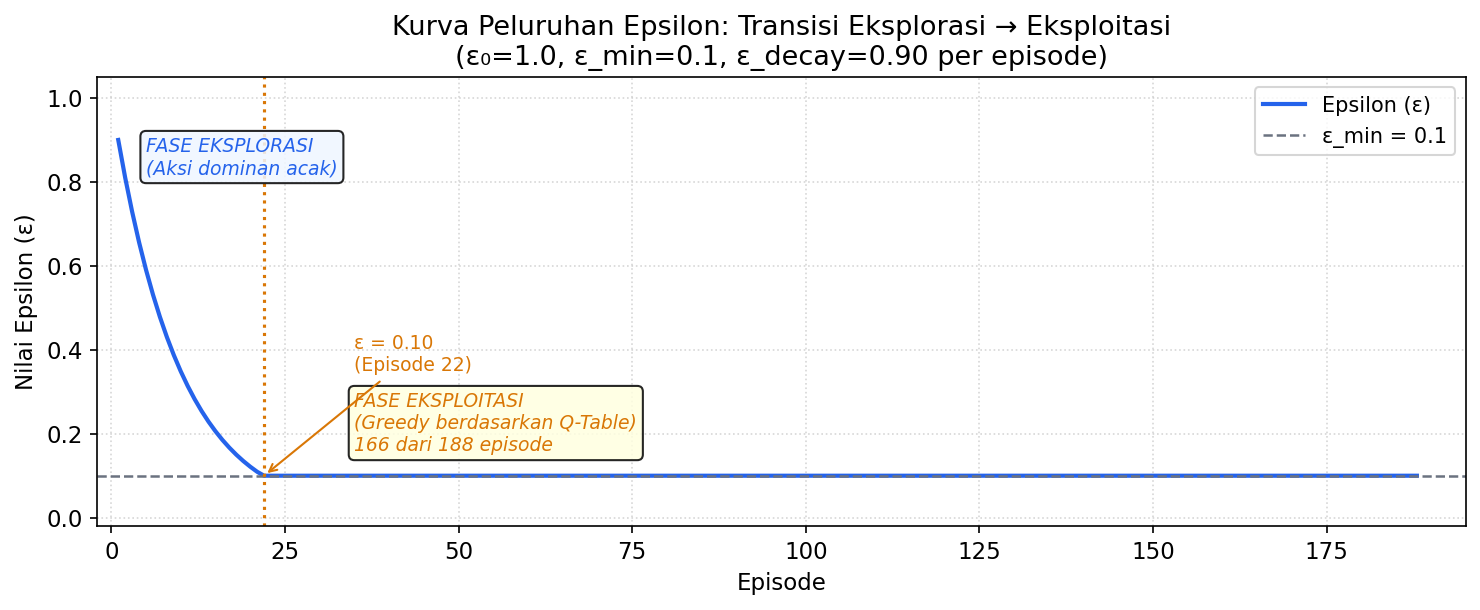
\includegraphics[width=0.85\textwidth]{gambar/epsilon_decay_ql.png} 
\caption{Kurva Peluruhan Epsilon ($\epsilon$-Greedy Decay) Agen Q-Learning}
\label{fig:epsilon_decay_ql}
\end{figure}

Berdasarkan analisis log lintasan aksi pada \texttt{log\_ql.csv}, proses pembelajaran agen secara garis besar terbagi ke dalam empat fase evolusi taktis. Dengan $\epsilon_{\text{decay}} = 0,90$, nilai $\epsilon$ menyentuh ambang minimum $0,10$ sekitar episode ke-22:
\begin{enumerate}
    \item \textbf{Fase 1: Rekognisi Stokastik (Episode 1--22):} Pada tahap ini, nilai $\epsilon$ masih di atas ambang minimum sehingga agen menyurvei berbagai \textit{endpoint} secara acak. Di fase ini, agen langsung berhasil mengidentifikasi celah-celah awal pada \textit{endpoint} 0 (\texttt{/search}) dan \textit{endpoint} 4 (\texttt{/login}). 
    \item \textbf{Fase 2: Eksploitasi Terarah Awal (Episode 23--300):} Setelah $\epsilon$ mencapai batas bawah ($0,10$), 90\% aksi dipilih berdasarkan $\arg\max Q(s,a)$. Agen secara intensif membombardir \textit{endpoint} 0 yang telah terbukti memberikan penguatan tinggi ($+50$). Setiap kali satu varian muatan SQLi atau XSS pada \textit{endpoint} 0 berhasil terverifikasi, aksi tersebut langsung di-mask, mendorong agen untuk mengeksploitasi muatan lain pada \textit{endpoint} yang sama. 
    \item \textbf{Fase 3: Pengalihan Ruang Serang dan Penemuan Celah Tersembunyi (Episode 301--787):} Setelah seluruh celah pada \textit{endpoint} 0 ter-mask, kebijakan $\arg\max$ agen terdorong beralih ke permukaan serang berikutnya. Di fase ini, agen berhasil menemukan 3 celah DOM XSS pada \textit{endpoint} 3 (\texttt{/track-order}) serta 3 kebocoran berkas \textit{poison null byte} pada \textit{endpoint} 1 (\texttt{/ftp/}). Seluruh 14 celah selesai dieksploitasi pada episode ke-787.
    \item \textbf{Fase 4: Kejenuhan Ruang Aksi dan Stabilitas Kebijakan (Episode 788--1.585):} Karena seluruh 14 aksi rentan telah di-mask permanen, agen tidak dapat lagi memperoleh reward $+50$. Agen terus mengeksplorasi sisa aksi yang ada dengan menerima umpan balik normal ($-1$). Stabilitas kurva pada fase ini membuktikan bahwa tidak terjadi osilasi kebijakan atau perilaku berulang yang merusak konvergensi.
\end{enumerate}

\subsection{Analisis Pertumbuhan Cumulative Reward dan Laju Efisiensi}

Dinamika akumulasi perolehan insentif agen Q-Learning sepanjang 1.585 episode interaksi divisualisasikan pada Gambar \ref{fig:cumulative_reward_ql}.

\begin{figure}[H]
\centering
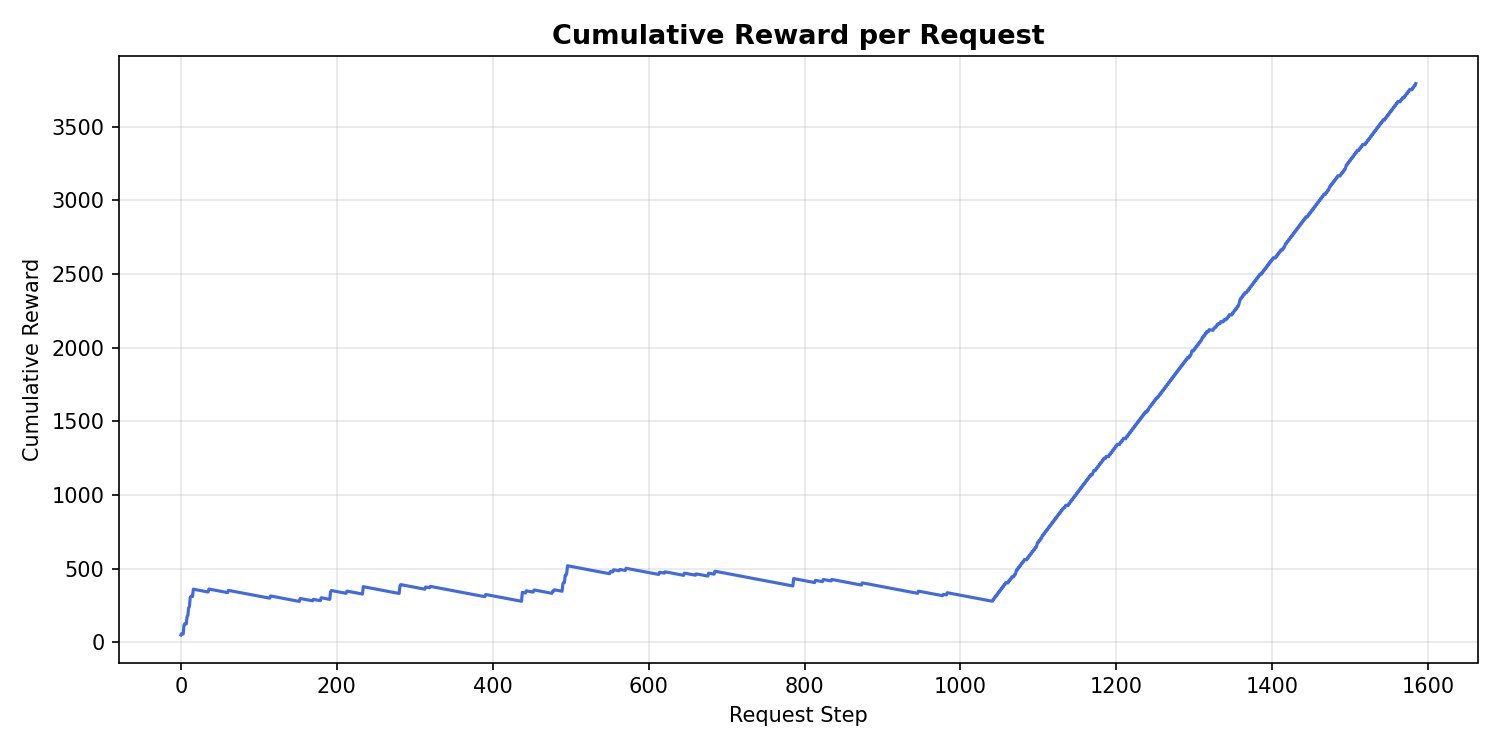
\includegraphics[width=0.85\textwidth]{gambar/cumulative_reward_ql.png} 
\caption{Kurva Pertumbuhan Cumulative Reward Q-Learning sepanjang 1.585 Episode}
\label{fig:cumulative_reward_ql}
\end{figure}

Kurva pada Gambar \ref{fig:cumulative_reward_ql} menunjukkan akumulasi reward hingga mencapai skor akhir \textbf{+3.783}. Lonjakan vertikal pada kurva berkorelasi langsung dengan episode di mana agen berhasil mengeksekusi celah keamanan baru ($+50$). Karakteristik kurva yang konsisten berada pada domain positif membuktikan bahwa insentif positif dari temuan kerentanan dan anomali jauh lebih dominan dibandingkan akumulasi penalti interaksi normal ($-1$). 

Laju akumulasi penemuan kerentanan disajikan pada Gambar \ref{fig:request_count_efficiency_ql}.

\begin{figure}[H]
\centering
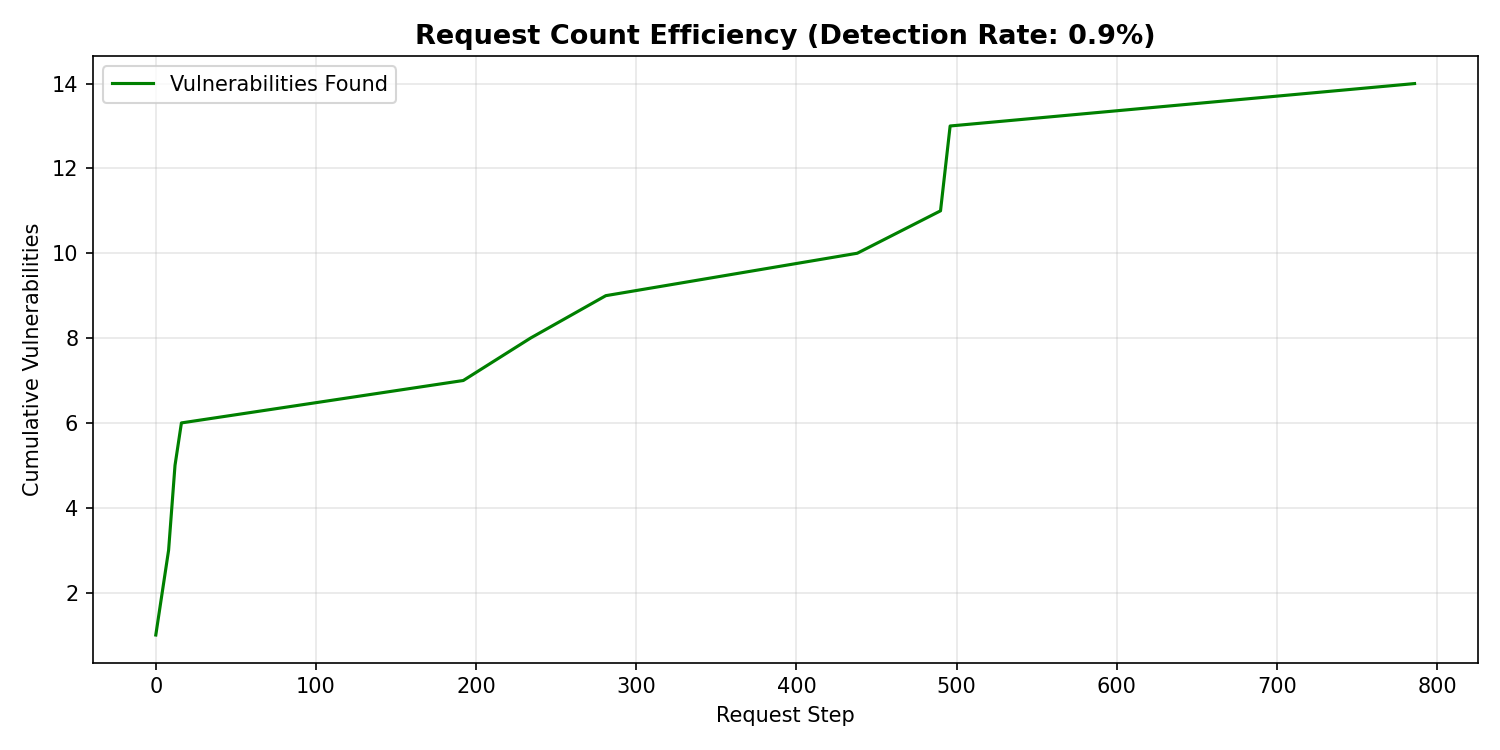
\includegraphics[width=0.85\textwidth]{gambar/request_count_efficiency_ql.png} 
\caption{Grafik Laju Penemuan Kerentanan Kumulatif Q-Learning (Efisiensi Request)}
\label{fig:request_count_efficiency_ql}
\end{figure}

Gambar \ref{fig:request_count_efficiency_ql} membuktikan bahwa agen Q-Learning tidak membutuhkan waktu pemanasan yang lama: celah pertama teridentifikasi pada \textbf{Episode 1}, dan seluruh 14 aksi rentan berhasil dituntaskan pada episode ke-787.

\subsection{Analisis Struktur Q-Table dan Nilai Q Tertinggi}

Sepanjang proses interaksi, agen Q-Learning memetakan lingkungan ke dalam \textbf{25 state unik} yang tercatat pada Q-Table. Tabel \ref{tab:qtable_top} menyajikan 10 nilai estimasi Q tertinggi yang dihasilkan pada akhir proses pelatihan. 

\begin{table}[H]
\centering
\caption{10 Nilai Q Tertinggi pada Q-Table Hasil Pelatihan Q-Learning}
\label{tab:qtable_top}
\begin{tabular}{|l|l|r|}
\hline
\textbf{Kondisi State} & \textbf{Aksi Terpilih (Payload@Endpoint)} & \textbf{Nilai Q} \\
\hline
\texttt{2xx|0|0|0|0|0|0|0} & \texttt{sqli\_comment@ep3} (\texttt{apple\textquotesingle --}) & 67,67 \\
\texttt{5xx|2|0|0|0|3|0|4} & \texttt{sqli\_login@ep0} (Bypass Login) & 59,18 \\
\texttt{2xx|0|0|0|0|6|0|0} & \texttt{sqli\_login@ep0} (Bypass Login) & 30,93 \\
\texttt{4xx|2|0|0|0|1|0|4} & \texttt{fuzz\_null@ep0} (\texttt{\%00}) & 30,89 \\
\texttt{4xx|1|0|0|0|1|0|4} & \texttt{sqli\_login@ep0} (Bypass Login) & 29,28 \\
\texttt{2xx|0|0|0|0|5|0|0} & \texttt{sqli\_login@ep0} (Bypass Login) & 29,04 \\
\texttt{4xx|0|0|0|0|4|0|4} & \texttt{fuzz\_null@ep1} (\texttt{\%00}) & 24,39 \\
\texttt{2xx|0|0|1|0|3|0|0} & \texttt{xss\_script@ep0} (\texttt{<script>}) & 14,94 \\
\texttt{2xx|2|0|1|0|2|0|0} & \texttt{sqli\_login@ep2} (Bypass Login) & 14,85 \\
\texttt{2xx|1|0|0|0|2|0|0} & \texttt{sqli\_login@ep0} (Bypass Login) & 11,69 \\
\hline
\end{tabular}
\end{table}

Nilai Q tertinggi yang tercatat pada tabel mencapai \textbf{67,67} pada \textit{state} \texttt{2xx|0|0|0|0|0|0|0}. Pola yang menonjol adalah dominasi aksi berbasis injeksi SQL seperti \texttt{sqli\_login@ep0} pada baris-baris teratas. Pola ini menunjukkan bahwa aksi tersebut memperoleh estimasi nilai tinggi pada state yang diamati. Interpretasi ini perlu dibaca bersama distribusi aksi dan hasil verifikasi, karena nilai Q sendiri bukan bukti kerentanan. Visualisasi peta panas (\textit{heatmap}) sebaran nilai Q pada seluruh pasangan \textit{state-action} disajikan pada Gambar \ref{fig:q_table_heatmap_ql}.

\begin{figure}[H]
\centering
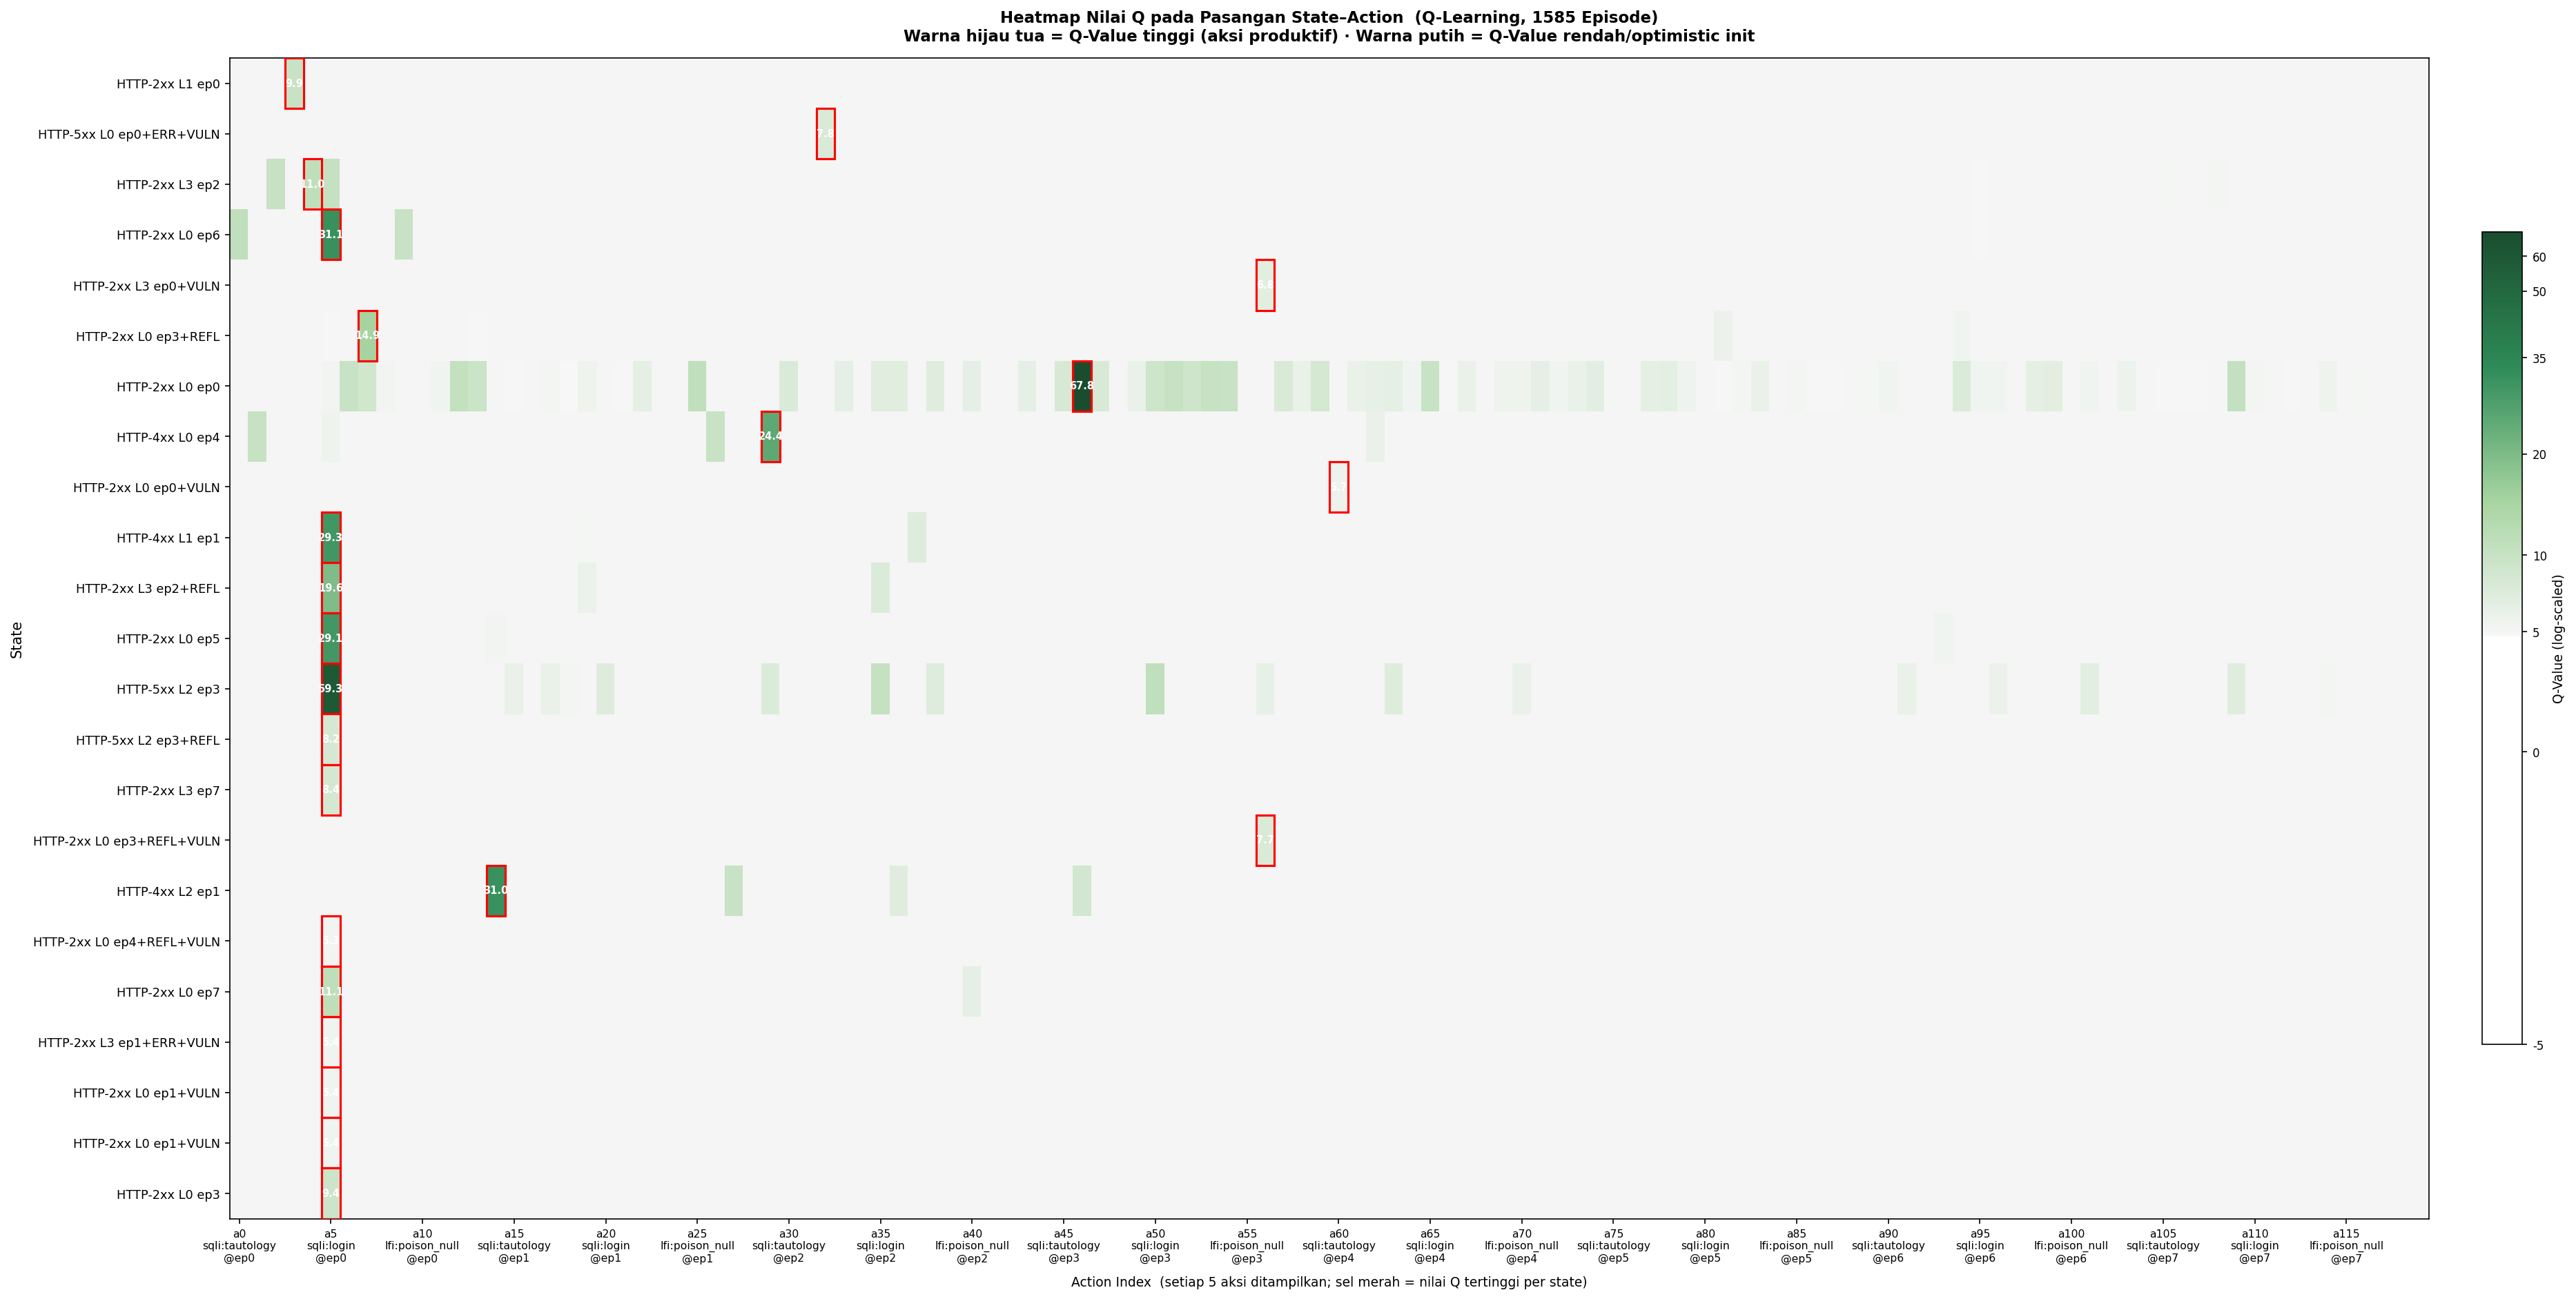
\includegraphics[width=0.95\textwidth]{gambar/q_table_heatmap_ql.png} 
\caption{Heatmap Matriks Q-Table: Pemetaan Nilai Aksi terhadap State Lingkungan}
\label{fig:q_table_heatmap_ql}
\end{figure}


\section{Evaluasi Komparatif: Tabular Q-Learning vs Deep Q-Network (DQN)}

\subsection{Perbandingan Kinerja Kuantitatif Q-Learning dan DQN}

Untuk memperkaya analisis kemampuan representasi kecerdasan buatan dalam pengetesan penetrasi web, sistem mengimplementasikan agen Deep Q-Network (DQN) sebagai pembanding terhadap agen tabular Q-Learning pada anggaran interaksi yang identik (1.585 episode). Tabel \ref{tab:comparison_ql_dqn} merangkum perbandingan kinerja kuantitatif antara kedua algoritma pemelajaran penguatan tersebut.

\begin{table}[htbp]
\centering
\caption{Perbandingan Kinerja Q-Learning vs Deep Q-Network (DQN)}
\label{tab:comparison_ql_dqn}
\small % Ukuran font proporsional
\setlength{\tabcolsep}{6pt} % Mengatur jarak antar kolom agar pas
\begin{tabular}{l c c}
\toprule
\textbf{Metrik Evaluasi} & \textbf{Tabular Q-Learning} & \textbf{Deep Q-Network (DQN)} \\
\midrule
Anggaran Permintaan Payload & 1.585 & 1.585 \\
Total Transaksi HTTP (\textit{w/ verifikasi}) & 1.639 & 1.636 \\ 
Kerentanan Terverifikasi Ditemukan & \textbf{14} & 13 \\ 
Jumlah Lokasi Kerentanan Unik & 5 & 5 \\
SQL Injection & 6 & 6 \\
Reflected XSS (DOM Verified) & 5 & 5 \\ 
Fuzzing / File Disclosure & 3 & 2 \\
Akumulasi Insentif (\textit{Cumulative Reward}) & 3.783 & \textbf{9.503} \\ 
Tingkat Keberhasilan (\textit{Vuln Hit Rate}) & 0,88\% & 0,76\% \\ 
Rasio Permintaan per Kerentanan & \textbf{113,21} & 121,92 \\ 
Episode Penemuan Pertama & Episode 1 & Episode 1 \\
Episode Seluruh Temuan Dikuasai & Episode 787 & \textbf{Episode 443} \\
Waktu Eksekusi Pelatihan & \textbf{142,55 detik} & 146,95 detik \\ 
\bottomrule
\end{tabular}
\end{table}

\subsection{Analisis Kemampuan Generalisasi Nilai dan Akumulasi Reward}

Data pada Tabel \ref{tab:comparison_ql_dqn} memperlihatkan perbedaan fundamental antara pendekatan tabular dan aproksimasi fungsi berbasis jaringan saraf tiruan:
\begin{enumerate}
    \item \textbf{Kecepatan Penemuan Kerentanan:} DQN berhasil mengidentifikasi seluruh 13 kerentanan yang ditemukannya (6 SQLi, 5 XSS, 2 Fuzz) secara jauh lebih cepat, yaitu pada \textbf{Episode 443}, dibandingkan Q-Learning yang membutuhkan 787 episode untuk menemukan 14 kerentanan. Hal ini dimungkinkan oleh kemampuan aproksimasi fungsi jaringan saraf yang mampu melakukan generalisasi nilai (\textit{value generalization}) lintas ruang \textit{state} vektor 28 dimensi. Ketika jaringan mempelajari bahwa suatu vektor input mencirikan anomali, bobot jaringan secara serempak memperbarui estimasi nilai untuk state-state berdekatan. 
    \item \textbf{Akumulasi Reward (+9.503 vs +3.783):} DQN mencatatkan perolehan \textit{cumulative reward} sekitar 2,51 kali lipat lebih besar dibanding Q-Learning. Mekanisme memori pengalaman (\textit{experience replay buffer}) berkapasitas 10.000 transisi memungkinkan sampel pengalaman berinsentif tinggi dilatih berulang kali (\textit{mini-batch sampling}) ke dalam bobot jaringan saraf, menjaga stabilitas estimasi nilai positif sepanjang proses pelatihan. 
\end{enumerate}

\subsection{Analisis Perbedaan Pola Eksplorasi: Konsentrasi vs Distribusi Merata}

Perbedaan yang sangat kontras juga tampak pada profil distribusi permintaan antar-\textit{endpoint}:
\begin{itemize}
    \item \textbf{Q-Learning Tabular:} Sangat terkonsentrasi secara tajam pada \textit{endpoint} 0 (1.184 dari 1.585 \textit{request}, atau 74,7\%). Tabel lookup Q-Learning memperbarui nilai secara terisolasi per sel $(s, a)$, sehingga begitu satu sel memperoleh nilai sangat tinggi, agen cenderung terus mengeksploitasi sel tersebut pada state aktif. 
    \item \textbf{Deep Q-Network (DQN):} Mengalokasikan permintaan yang jauh lebih tersebar dan merata di seluruh 8 \textit{endpoint} (berkisar antara 73 hingga 377 \textit{request} per \textit{endpoint}). Hal ini dipengaruhi oleh laju peluruhan eksplorasi yang lebih landai ($\epsilon_{\text{decay}} = 0,9965$) yang mempertahankan tingkat eksplorasi aktif hingga episode ke-1.000. 
\end{itemize}

Grafik kurva pertumbuhan insentif dan laju efisiensi DQN masing-masing disajikan pada Gambar \ref{fig:cumulative_reward_dqn} dan Gambar \ref{fig:request_count_efficiency_dqn}.

\begin{figure}[H]
\centering
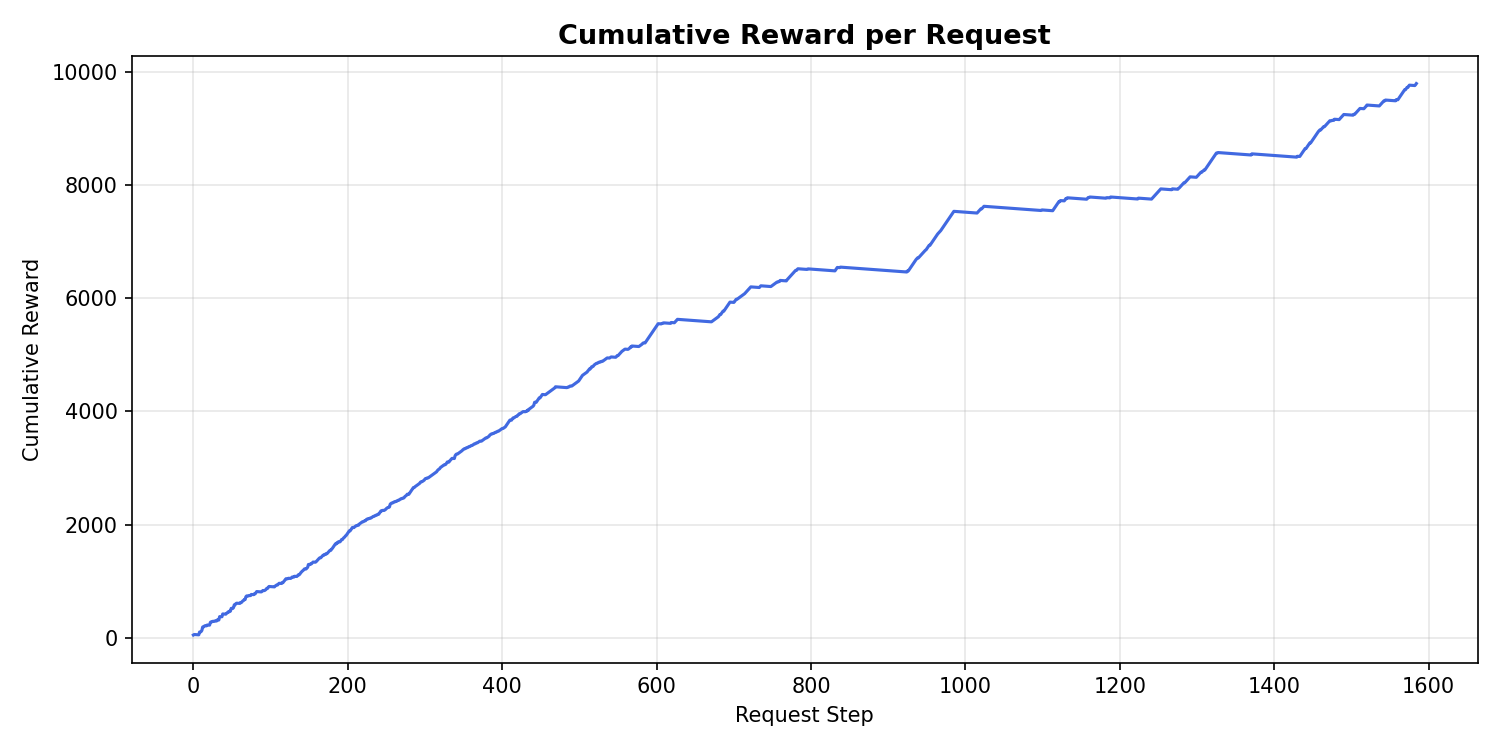
\includegraphics[width=0.85\textwidth]{gambar/cumulative_reward_dqn.png} 
\caption{Kurva Pertumbuhan Cumulative Reward Deep Q-Network (DQN)}
\label{fig:cumulative_reward_dqn}
\end{figure}

\begin{figure}[H]
\centering
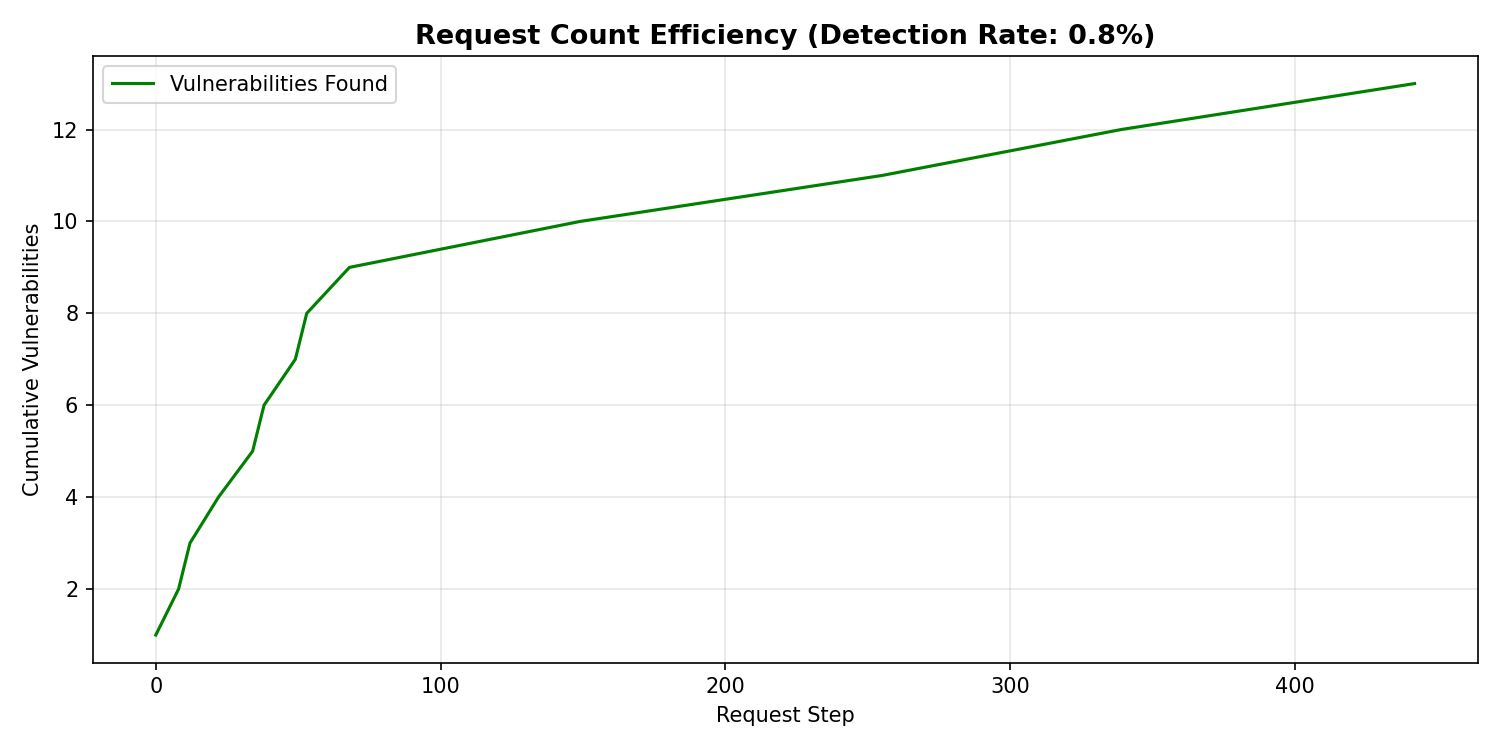
\includegraphics[width=0.85\textwidth]{gambar/request_count_efficiency_dqn.png} 
\caption{Grafik Laju Penemuan Kerentanan Kumulatif Deep Q-Network (DQN)}
\label{fig:request_count_efficiency_dqn}
\end{figure}

\text Hasil menunjukkan perbedaan kinerja pada run yang diamati. Q-Learning menemukan 14 aksi terverifikasi (7 SQLi, 5 XSS, 2 Fuzz), sedangkan DQN menemukan 13 aksi (6 SQLi, 5 XSS, 2 Fuzz). DQN mencapai seluruh temuan yang diperolehnya pada episode ke-443, sementara Q-Learning mencapai 14 temuan pada episode ke-787. Reward kumulatif masing-masing adalah 3.783 dan 9.503. Nilai reward yang lebih tinggi tidak dengan sendirinya menunjukkan deteksi yang lebih baik; hasil ini perlu dibaca bersama jumlah temuan, anggaran request, serta sifat evaluasi yang in-sample. Durasi pelatihan yang tercatat masing-masing 142,55 detik dan 146,95 detik pada run ini.
\section{Perbandingan dengan OWASP ZAP}

\subsection{Rincian Arsitektur dan Prosedur Pemindaian OWASP ZAP}

Pada eksperimen ini, OWASP ZAP dijalankan sebagai daemon yang dikendalikan melalui API oleh skrip Python. Alurnya terdiri atas pengendali eksperimen, API ZAP, mesin pemindaian, aplikasi target, dan pengolahan alert. Pengendali menentukan URL dan tahapan pemindaian. Mesin ZAP menjalankan akses URL, spider, serta pemindaian aktif. Hasil pesan dan alert kemudian diambil kembali oleh pengendali untuk dihitung menggunakan kriteria penelitian.

\begin{enumerate}
    \item \textbf{Pengendali Python:} menetapkan dua URL dalam cakupan, memeriksa versi ZAP, mencatat jumlah pesan awal, dan mengirim perintah melalui API.
    \item \textbf{Core API ZAP:} menyediakan operasi untuk mengakses URL, memulai spider dan pemindaian aktif, membaca status proses, mengambil riwayat pesan, serta mengambil alert.
    \item \textbf{Akses URL dan spider:} setiap URL diakses terlebih dahulu. Spider kemudian menelusuri sumber daya yang dapat dijangkau dan statusnya diperiksa secara berkala sampai proses selesai.
    \item \textbf{Pemindaian aktif:} setelah spider selesai, pemindaian aktif dijalankan dengan \texttt{recurse=false}. ZAP mengirimkan permintaan uji sesuai aturan dan konfigurasi pemindainya.
    \item \textbf{Pengumpulan hasil:} setelah setiap tahap, skrip membaca jumlah pesan dan menghitung selisihnya terhadap jumlah sebelum tahap tersebut. Setelah pemindaian selesai, skrip mengambil alert melalui API.
    \item \textbf{Penyaringan untuk analisis:} alert dikelompokkan menurut kategori penelitian. Hanya alert SQLi, XSS, atau path traversal dengan risiko High atau Medium yang dihitung sebagai temuan relevan.
\end{enumerate}

Untuk memberikan representasi visual yang jelas mengenai interaksi sistem, hubungan komponen arsitektur modular OWASP ZAP beserta alur prosedur pemindaian yang dikendalikan oleh skrip pengendali Python tersebut dimodelkan pada Gambar \ref{fig:zap_architecture_flow}.

\begin{figure}[H]
\centering
% Memaksa seluruh diagram mengecil secara otomatis mengikuti lebar teks halaman dokumen
\resizebox{\textwidth}{!}{
\begin{tikzpicture}[
    font=\sffamily\small,
    node distance=1.2cm and 1.5cm,
    % Definisi Gaya Kotak Komponen
    core/.style={rectangle, rounded corners, draw=blue!70, fill=blue!10, thick, minimum width=3.3cm, minimum height=1.1cm, align=center},
    scanner/.style={rectangle, rounded corners, draw=orange!70, fill=orange!10, thick, minimum width=3.3cm, minimum height=1.1cm, align=center},
    db/.style={cylinder, draw=gray!70, fill=gray!20, thick, shape border rotate=90, minimum width=2.2cm, minimum height=1.6cm, align=center},
    external/.style={rectangle, draw=green!70!black, fill=green!5, thick, minimum width=3.3cm, minimum height=1.1cm, align=center},
    % Definisi Gaya Garis Panah
    arrow/.style={- {Stealth[scale=1.2]}, thick, draw=gray!80},
    doublearrow/.style={{Stealth[scale=1.2]} - {Stealth[scale=1.2]}, thick, draw=gray!80}
]

    % --- LAYER 1: PENGENDALI PYTHON ---
    \node[external] (python) {\textbf{1. Pengendali Python}\\(Skrip Eksperimen)};
    
    % --- LAYER 2: INTERFACES ZAP ---
    \node[core] (api) [right=2.2cm of python] {\textbf{2. Core API ZAP}\\(Endpoint Operasi)};
    \node[core] (engine) [right=1.2cm of api] {\textbf{ZAP Core Engine}\\(Orkestrator Sesi)};

    % --- LAYER 3: PROSEDUR PEMINDAIAN ---
    \node[scanner] (spider) [above right=0.4cm and 1.2cm of engine] {\textbf{3. Akses \& Spider}\\(Pemetaan Direktori)};
    \node[scanner] (active) [below right=0.4cm and 1.2cm of engine] {\textbf{4. Pemindaian Aktif}\\(Active Scanner)};

    % --- LAYER 4: TARGET & REPOSITORI ALERTS ---
    \node[external] (target) [right=4.2cm of engine] {\textbf{Aplikasi Target}\\(Subset 2 Endpoint)};
    \node[db] (database) [below=1.4cm of engine] {\textbf{5 \& 6. Filter Alerts}\\(High / Medium Only)};

    % --- ALUR DATA DAN HUBUNGAN ANTAR KOMPONEN ---
    % Pengendali mengirim perintah ke API
    \draw[arrow] (python) -- node[above, font=\footnotesize] {Kendalikan} 
                            node[below, font=\footnotesize] {Skrip API} (api);
    
    % API meneruskan ke Core Engine ZAP
    \draw[doublearrow] (api) -- (engine);
    
    % Core Engine menggerakkan tahapan operasional
    \draw[arrow] (engine) |- (spider);
    \draw[arrow] (engine) |- (active);
    
    % Aktivitas pemindaian dari modul ke target
    \draw[arrow] (spider) -| node[pos=0.4, above, font=\footnotesize] {Akses URL} (target);
    \draw[arrow] (active) -| node[pos=0.4, below, font=\footnotesize] {1.585 Request} (target);
    
    % Pengumpulan kembali hasil alert ke database
    \draw[arrow] (engine) -- (database);
    
    % Alur pengambilan temuan kembali ke skrip python pengendali
    \draw[arrow] (database) -| node[pos=0.8, left, font=\footnotesize, xshift=-0.2cm] {Ambil Temuan} (python);

\end{tikzpicture}
} % Akhir penutup \resizebox
\caption{Rincian Arsitektur Integrasi Pengendali Python dan Prosedur Pemindaian OWASP ZAP}
\label{fig:zap_architecture_flow}
\end{figure}



Pemindai pasif ZAP menganalisis pesan yang diamati tanpa mengubah pesan, sedangkan pemindai aktif mengirimkan probe ke target. Skrip eksperimen secara eksplisit menjalankan akses URL, spider, dan pemindaian aktif; skrip tidak memulai pekerjaan pemindaian pasif tersendiri. Alert yang tidak masuk kriteria perbandingan tetap merupakan keluaran ZAP, tetapi tidak dihitung sebagai temuan relevan dalam metrik penelitian.

Laporan pemindaian terkontrol yang digunakan mencatat ZAP versi 2.17.0 dan menghasilkan total akumulasi lalu lintas komunikasi sebanyak 1.585 request pesan pada target yang mencakup aktivitas pemetaan akses URL, spider, serta eksekusi pemindaian aktif. Dari seluruh rangkaian aktivitas tersebut, ZAP menghasilkan 32 alert mentah di mana terdapat dua alert yang memenuhi kriteria batas risiko High atau Medium untuk dihitung ke dalam temuan relevan perbandingan. Pengklasifikasian ini wajib dipastikan konsistensinya di sepanjang penyebutan metrik ZAP pada Bab 4.

Pada subset dua endpoint yang sama, QL mencatat 1.214 permintaan payload untuk 10 temuan, sedangkan ZAP mencatat total 1.585 request pesan untuk menghasilkan dua temuan relevan. Cakupan endpoint yang sama tidak membuat prosedur kedua metode sepenuhnya setara. QL memilih payload satu per satu melalui kebijakan agen, sedangkan ZAP menjalankan alur akses URL, spider, dan pemindaian aktif. Karena strategi dan cara penghitungan request berbeda, rasio request per temuan hanya bersifat deskriptif untuk eksperimen ini.

Perbandingan dengan OWASP ZAP dilakukan menggunakan hasil pemindaian terkontrol pada dua endpoint, yaitu \texttt{/rest/products/search?q=} dan \texttt{/ftp/}. Untuk membatasi perbedaan cakupan, hasil Q-Learning juga dihitung pada subset dua endpoint tersebut. Ringkasan perbandingan ditampilkan pada Tabel \ref{tab:zap_comparison}.

\begin{table}[H]
\centering
\caption{Perbandingan Hasil Q-Learning dan OWASP ZAP pada Dua Endpoint}
\label{tab:zap_comparison}
\begin{tabular}{|l|c|c|}
\hline
\textbf{Metrik} & \textbf{Q-Learning (subset)} & \textbf{OWASP ZAP} \\
\hline
Endpoint yang dicakup & 2 & 2 \\
Jumlah request & 1.226 & 1.585 \\
Temuan relevan yang dihitung & 10 & 2 \\
SQL Injection & 5 & 1 \\
Reflected XSS & 2 & 1 \\
Fuzzing / anomali file & 3 & 0 \\
Request per temuan & 122,60 & 792,50 \\
\hline
\end{tabular}
\end{table}

Pada subset tersebut, rasio request per temuan Q-Learning adalah 122,60, sedangkan OWASP ZAP sebesar 792,50. Rasio kedua nilai tersebut sekitar 6,46. Angka ini menggambarkan hasil pada konfigurasi dan run yang digunakan dalam penelitian, bukan bukti bahwa Q-Learning secara umum 6,46 kali lebih efisien. ZAP dan Q-Learning menggunakan strategi pemindaian serta kumpulan payload yang berbeda. Karena itu, perbandingan ini bersifat deskriptif dan perlu ditafsirkan dengan mempertimbangkan perbedaan metode.

OWASP ZAP menghasilkan 32 alert mentah; dua alert masuk kategori yang dihitung sebagai temuan relevan dalam laporan perbandingan, yaitu satu SQL Injection dan satu Reflected XSS. Alert lainnya tidak dimasukkan ke hitungan kerentanan aktif pada penelitian ini. Gambar \ref{fig:vuln_breakdown} menyajikan distribusi temuan berdasarkan kategori.

\begin{figure}[H]
\centering
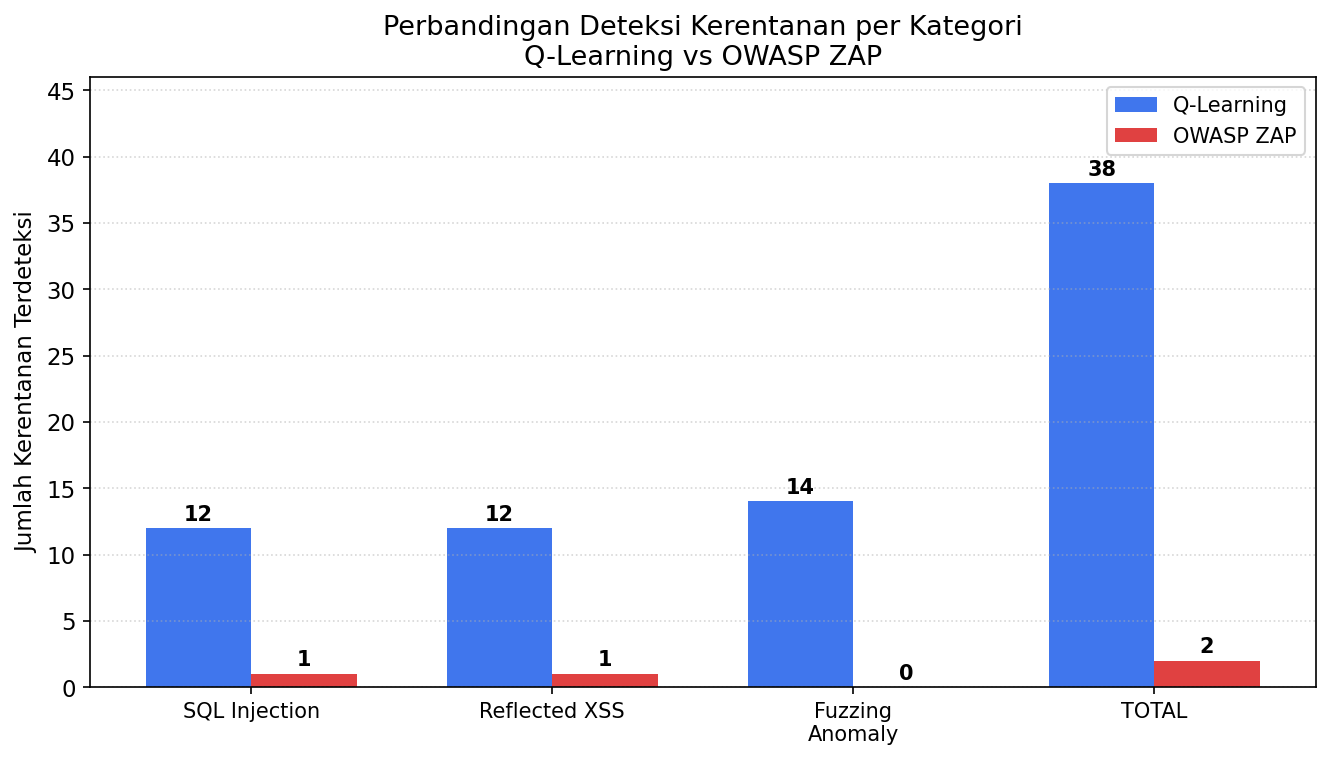
\includegraphics[width=0.85\textwidth]{gambar/vuln_breakdown_ql_zap.png}
\caption{Distribusi Temuan Relevan Q-Learning dan OWASP ZAP}
\label{fig:vuln_breakdown}
\end{figure}



\section{Keterbatasan Penelitian}

Hasil penelitian ini memiliki beberapa batasan. Pertama, metrik Q-Learning dan DQN bersifat \textit{in-sample}: metrik dihitung dari episode yang juga digunakan selama pelatihan. Oleh sebab itu, hasil belum mengukur kemampuan generalisasi kebijakan pada data uji terpisah maupun aplikasi web lain. Kedua, percobaan yang dilaporkan menggunakan satu nilai \textit{random seed}; variasi antar-run belum dianalisis sehingga perbedaan kinerja belum dapat dinyatakan signifikan secara statistik.

Ketiga, daftar payload dan pemetaan \textit{surface} disusun dengan pengetahuan tentang struktur OWASP Juice Shop. Hal ini merupakan \textit{human prior} yang perlu dinyatakan sebagai bagian dari metode penelitian. Keempat, label ground truth dan mekanisme verifikasi memakai bukti teknis yang sejenis dengan sistem, sehingga benchmark detektor tidak sepenuhnya independen. Hasil benchmark sebaiknya dipahami sebagai konsistensi terhadap ground truth terkurasi, bukan bukti akurasi universal.

Kelima, perbandingan dengan OWASP ZAP hanya mencakup dua endpoint dan menggunakan strategi pemindaian yang berbeda. Jumlah request dan temuan karena itu tidak sepenuhnya setara. Penelitian lanjutan dapat mengulang eksperimen dengan beberapa seed, menyediakan evaluasi held-out, menguji target tambahan, dan menyamakan prosedur penghitungan request serta temuan.

Pada eksperimen yang dilakukan, Q-Learning memperoleh 14 temuan terverifikasi dan DQN memperoleh 13 temuan terverifikasi dari anggaran masing-masing 1.585 request payload. Benchmark detektor pada 120 aksi menghasilkan 13 \textit{true positive}, 1 \textit{false negative}, 0 \textit{false positive} pada 60 aksi berlabel negatif, serta 46 aksi berstatus \textit{unknown}. Perbandingan terbatas pada dua endpoint menunjukkan 10 temuan Q-Learning dan 2 temuan ZAP, tetapi perbedaan metode pemindaian membatasi kesimpulan efisiensi yang dapat ditarik. Seluruh hasil tersebut berlaku pada lingkungan dan konfigurasi penelitian ini.


